\documentclass[notitlepage]{report}

\usepackage{titling}
\usepackage{subcaption}
\usepackage{amsmath}
\usepackage{url}
\usepackage{wrapfig}
\usepackage{amssymb}
\usepackage{breqn}
\usepackage[a4paper, total={6in, 9in}]{geometry}
\newcommand\norm[1]{\left\lVert#1\right\rVert}
\newcommand{\angstrom}{\text{\normalfont\AA}}
\usepackage{natbib}
\usepackage{caption}
\usepackage{graphicx}
\usepackage{siunitx}
\usepackage{hyperref}
\graphicspath{ {./images/} }

\title{Numerical Simulations and Analytical Results Exploring the use of the Generalized Langevin Equation for Simulations of Atomic Scale Surface Dynamics}
\author{Blind Grading Number: 4631L \\[0.3cm]{Supervised by Dr. John Ellis}}
\date{17th of May 2021}

\newcommand{\mev}{\si{\milli\eV}}
\newcommand{\thz}{\si{\tera\hertz}}
\newcommand{\ns}{\si{\nano\second}}
\newcommand{\ps}{\si{\pico\second}}
\newcommand{\ips}{\si{\per\pico\second}}
\newcommand{\fs}{\si{\femto\second}}
\newcolumntype{P}[1]{>{\centering\arraybackslash}p{#1}}
\newcolumntype{P}[1]{>{\centering\arraybackslash}p{#1}}
\newcolumntype{P}[1]{>{\centering\arraybackslash}p{#1}}
\newcolumntype{P}[1]{>{\centering\arraybackslash}p{#1}}
\newcommand{\expnumber}[2]{{#1}\mathrm{e}{#2}}

\begin{document}
\maketitle
\thispagestyle{empty}

\begin{abstract}

	Langevin equations are widely used as a computationally cheap model of a subset of the degrees of freedom in a complex system. The white noise present in the original Langevin equation, while often a good approximation, does not capture the colored noise in most real systems. This necessitates the introduction of the generalized Langevin equation (GLE). Recent results in the field of surface dynamics \cite{Ward} have used the GLE to explain experimental data for the activated diffusion of lithium on copper(111) by introducing band-limited noise. However, the noise spectrum required was band-limited to around $\SI{1.25}{\thz}$, much lower than the $\SI{7.4}{\thz}$ \cite{sinha} which the phonon cutoff frequency of copper would suggest. The following report presents a careful evaluation of the performance of the GLE in the presence of a corrugated background potential through analytic analysis and numerical comparison with full 3D molecular dynamics (MD) simulations. The analytic work provides an interpretation of the parameters in the GLE in the wide bandwidth regime and proposes a simple technique for the extraction of parameters from experimental/MD results. A semi-realistic classical MD simulation of lithium on copper(111) is constructed with the correct copper phonon spectrum. The GLE with a frequency cutoff of $\SI{7.4}{\thz}$ is shown to reproduce the simulated MD results extremely well leading to the proposal that an additional, unknown, noise filter is present in lithium on copper(111) which reduces the effective bandwidth seen by the lithium. Since lithium is an extremely light atom with a thermal de Broglie wavelength on the order of $\SI{0.5}{\angstrom}$ at $\SI{140}{\kelvin}$, this filter may be quantum mechanical in nature.  

\end{abstract}


\vspace{1cm}
\begin{center}
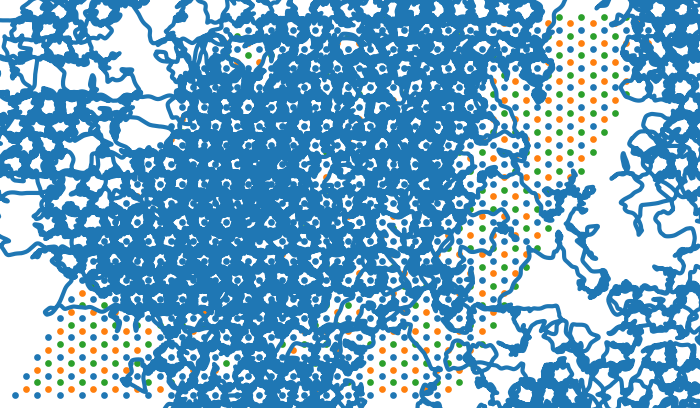
\includegraphics[width=0.80\textwidth]{md_top_down}
\end{center}

\pagebreak

\section*{Acknowledgments}

I would like to thank my supervisor, Dr. John Ellis, for the time, effort and enthusiasm he has invested in this project.
I would like to thank the Skye Foundation, Oppenheimer Memorial Trust and Cambridge Trust for providing the financial means for me to pursue the degree for which this report was submitted.

\addvspace{2cm}

\section*{Statement of Authenticity}

Except where specific reference is made to the work of others, this work is original and has not been already submitted either wholly or in part to satisfy any degree requirement at this or any other university.

\addvspace{2cm}

\section*{List of Acronyms}

\begin{itemize}
  \item GLE - Generalized Langevin equation
  \item MD - Molecular dynamics simulation
  \item HSEM - Helium spin echo microscopy
  \item ISF - Intermediate scattering function
  \item fcc - Face centered cubic crystal
  \item dof - Degrees of freedom
\end{itemize}

\tableofcontents
\listoffigures
\listoftables

\chapter{Introduction}

\section{Langevin Equations}

\subsection{The Langevin Equation} \label{sec:langevin_equation}

The Langevin equation provides a mechanism for studying certain complex many-body systems by focusing in on a single particle and treating the effect of other particles as stochastic. Following the derivations of Kubo \cite{Kubo}, this approach leads to the Langevin equation, a stochastic differential equation of the form 
\\
$$
m\ddot{\vec{r}}(t) + m \eta \dot{\vec{r}}(t) = \vec{f}(t)
$$
\\
where $\vec{r}(t)$ is the trajectory of a particle of mass $m$, $\eta$ is a friction constant in units of inverse time and $\vec{f}(t)$ is a stochastic force. It is often assumed that $\vec{f}(t)$ is isotropic, as well as uncorrelated for different times and directions. This is summarized through the relation 
\begin{equation}
\left<f_i(t)f_j(t')\right>=\sigma^2\delta(t-t')\delta_{ij} \label{eq:tdomain_corr}.
\end{equation}
The standard deviation $\sigma$ is given by the fluctuation dissipation theorem \cite{Kubo}, $\sigma^2=2k_BTm\eta$ where $k_B$ is the Boltzmann constant and $T$ is the temperature of the system. The friction term $m \eta \dot{\vec{r}}(t)$ counteracts the energy gain from the stochastic force to ensure the equipartition theorem holds. 

\subsection{The Generalized Langevin Equation}

Some of the assumptions made in the formulation of the Langevin equation do not hold for most real systems. The Fourier transform of \ref{eq:tdomain_corr} results in the expression
\begin{equation}
\left<\tilde{f}_i(\omega)\tilde{f}_j(\omega')\right>=2\pi\sigma^2\delta(\omega+\omega')\delta_{ij}. \label{eq:wdomain_corr}
\end{equation}
This equation tells shows that the power spectrum of the noise force is constant and does not fall off as $\omega \rightarrow \infty$. While this may be a reasonable approximation for many systems, all real system are band limited and therefore exhibit `colored' noise. One may introduce colored noise into the Langevin equation while maintaining the relations \ref{eq:tdomain_corr} and \ref{eq:wdomain_corr} by convolving $\vec{f}(t)$ with a memory kernel $K(t)$. The second fluctuation dissipation theorem \cite{Kubo}, requires a corresponding modification to the friction term which gives us the generalized Langevin equation (GLE)
\begin{equation}
m\ddot{\vec{r}} + m \eta \int dt' K\left(t-t'\right) \dot{\vec{r}}(t') = \int dt' K\left(t-t'\right) \vec{f}(t').
\end{equation}

\subsection{Including Background Potentials} \label{sec:gle_with_background}

If one views the GLE as simple stochastic generalization of Newton's second law, it is simple to add a term to the GLE to include the effect of a position dependent background potential $V(\vec{r})$,
\begin{equation}
m\ddot{\vec{r}} + m \eta \int dt' K\left(t-t'\right) \dot{\vec{r}}(t') + \nabla V\left(\vec{r}\right)= \int dt' K\left(t-t'\right) \vec{f}(t').
\end{equation}
\\
While this approach is very straight forward, it is not immediately obvious that the relation $\sigma^2 = 2k_BTm\eta$ guarantees thermalization in the presence of an arbitrary background potential. The various derivation of the GLE \cite{Kubo, Pathria, Tong} focus exclusively on the case of $V(x)=0$. Nevertheless, Langevin equations are frequently used in contexts where background potentials are necessary and justification for their use is either omitted or provided retroactively through comparison of results with independent sources \cite{Ward, Townsend, AVIDOR2019145}.  

\section{Surface Dynamics and Helium Spin-Echo Microscopy}

The field of surface dynamics aims to measure and model the motion of particles (referred to as `adatoms') adsorbed on the surface of various solid crystalline materials so as to better understand processes such as catalysis or the production of nanomaterials \cite{B810769F}. The field has adopted simulations of the GLE as a computationally efficient tool for studying its dynamical processes \cite{Ward, Townsend, AVIDOR2019145}. The rich experimental data available in the literature provides a setting in which the GLE can be applied to the same system across a wide range of length and time scales \cite{JARDINE2009323, HSEM}.

\subsection{The Cambridge Helium Spin-Echo Spectrometer}

\begin{figure}
	\centering
	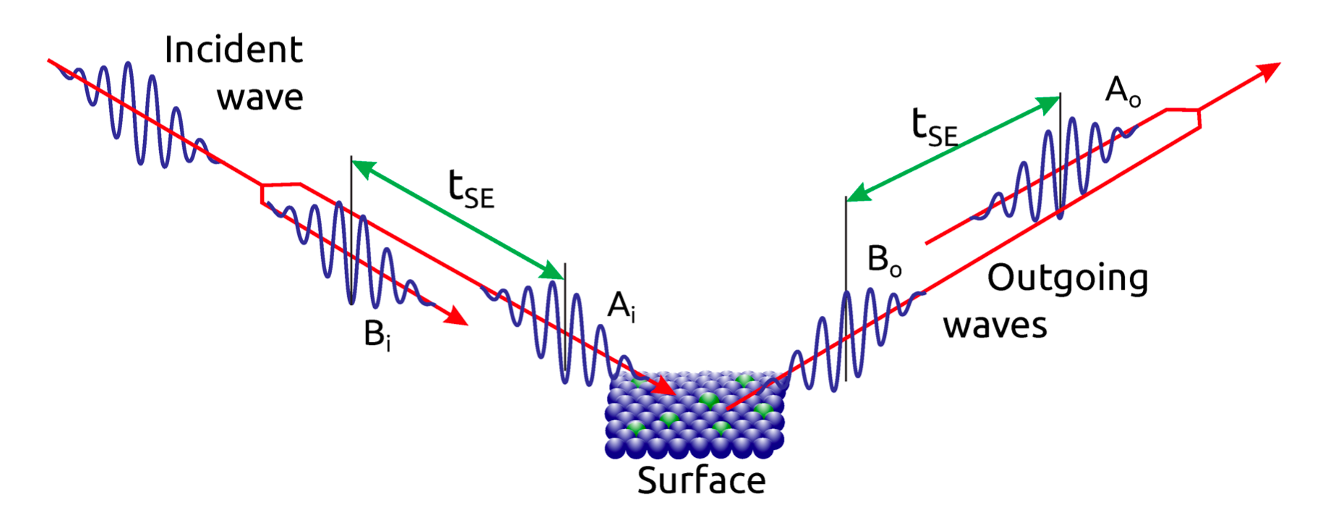
\includegraphics[width=0.8\textwidth]{hsem_schematic}
	\caption{Schematic of the helium spin-echo technique sourced from \cite{B810769F}. An incident spin-polarized helium wave packet is split into two components which strike the surface at distinct times separated by $t_{SE}$. Motion of the adatoms on the surface which occurs in this time affect the polarization of the scattered helium which may be used to construct the ISF of the motion.}
	\label{fig:hsem}
\end{figure}

The Cambridge helium spin-echo spectrometer probes the dynamics of adsorbates on the surface of a substrate using a beam of He-3 atoms scattered off the substrate surface. The spectrometer provides a measurement of the so called intermediate scattering function (discussed further in Section \ref{sec:isf_intro}) of an adsorbate's motion. The core principles of helium spin-echo microscopy (HSEM) are summarized in Figure \ref{fig:hsem} and its implementation is explored in further detail in \cite{Ward, HSEM, JARDINE2009323}.

\subsection{The Intermediate Scattering Function} \label{sec:isf_intro}

A quantity of interest in many surface scattering experiments is the so called intermediate scattering function (ISF) \cite{HSEM, JARDINE2009323, Ward}. The ISF is defined in terms of the Van Hove pair correlation function. For a single adatom, the van Hove pair correlation function coincides with the probability, $P(\vec{r}, t)$, of finding the particle at the position $\vec{r}$ at time $t$ given that the particle was present at the origin at $t=0$ \cite{vanhove} \footnote{This definition strictly speaking only applies when a single adatom is present on the surface. For more details see \cite{vanhove}.}. The ISF is then defined as the spatial Fourier transform of $P\left(\vec{r}, t\right)$,
\begin{equation}
	ISF\left(\Delta{\vec{K}}, t\right) = \int d\vec{r} e^{-i\Delta{\vec{K}}\cdot\vec{r}} P\left(\vec{r}, t\right).
\end{equation}
Within the context of a surface scattering experiment, the argument $\Delta{\vec{K}}$ is often referred to as `the momentum transfer' as this quantity corresponds to the momentum transferred to the surface in the process of scattering. The Cambridge HSEM device is largely insensitive to momentum transfer perpendicular to the surface as motion on the surface in this direction occurs at frequencies which exceed its working range \cite{HSEM}. The ISF is therefore often only quoted in terms of the 2D parallel component of the momentum transfer. 

\subsection{Adsorbate Motion}

Although effectively confined to motion on a 2D plane, adatoms may exhibit various sophisticated forms of motion. Typical motion observed in real systems include 2D diffusion, ballistic motion across the surface and hopping between regularly spaced absorption sites \cite{Ward, Townsend}. The type of dynamics an adsorbate exhibits is influenced by factors such as the details of the adsorbate-substrate interaction, the crystalline structure of atoms in the substrate, the temperature of the system as well as the density of the adatoms on the surface \cite{Ward, Townsend}. 

The motion of an adsorbate may vary over different timescales. Consider an adatom which spends most of its time oscillating about its local equilibrium in an absorption site but every so often obtains the energy to jump over to a neighboring absorption site. On short timescales (less than its typical oscillation period), the motion appears Brownian as the adatom randomly moves about the local patch of its potential well. At somewhat larger timescales, the particle will appear to oscillate about its potential well at some frequency approximately given by the curvature of the local equilibrium. On the longest time scales the particle appears to hop between well defined absorption sites. The signature of the motion on the different timescales is imprinted on the ISF and may be extracted with suitable analysis \cite{Ward}.

\pagebreak

\section{Lithium on Copper 111}

\begin{figure}
	\centering
	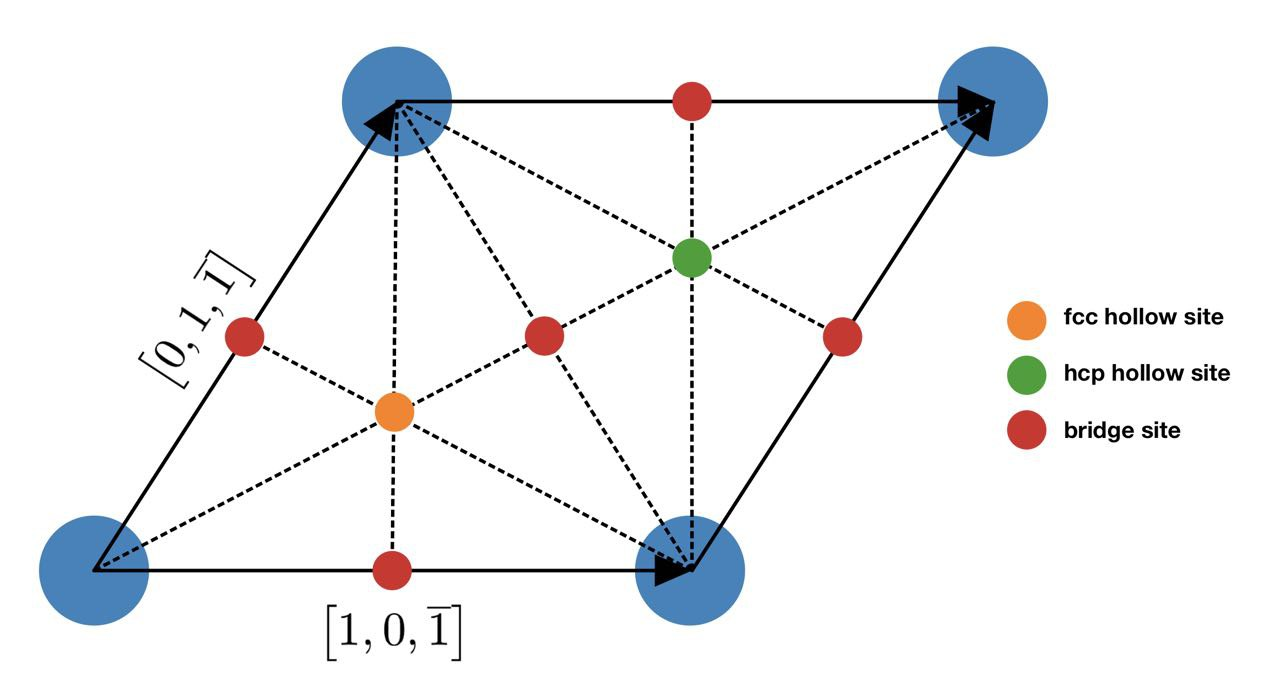
\includegraphics[width=0.8\textwidth]{primitive_cell}
	\caption{The unit cell which tiles a copper(111) surface. Lithium adsorbed on the surface is observed to sit within the two types of hollow sites and hop between sites with an activation energy of approximately $8\mev$ \cite{Ward}.}
	\label{fig:fcc_111_unit_cell}
\end{figure}

Previous work has used the GLE to explain the dynamic processes of Lithium adsorbed on copper(111) \cite{Ward}. Copper crystals have a face centered cubic (fcc) crystal structure and the 111 surface is tiled by the unit cell shown in Figure \ref{fig:fcc_111_unit_cell}. The experimental HSEM ISFs for lithium on copper(111) shows signs of activated diffusion at $\SI{140}{\kelvin}$ and previous work has concluded that the ISFs can be entirely reproduced through a GLE simulation with a band limited noise spectrum \cite{Ward}. The 3D molecular dynamics simulation presented in this report is modeled on this system to investigate the origin of this band limited noise spectrum. 

\chapter{Analytic Expressions for the GLE in a Harmonic Well and the Interpretation of GLE Parameters} \label{sec:gle_interpretation}

The discussion of the GLE in a background potential begins in the simple case of a harmonic well of natural frequency $\omega_0$, $V\left(x\right) = \frac{1}{2}m\omega_0^2x^2$. Using the statistical properties of the stochastic force, Appendix \ref{apx:analytic_gle_appendix} provides a first-principles derivation of the kinetic energy auto-correlation function and ISF of a particle in a harmonic well with an arbitrary memory kernel. The derivation introduces the Green's function of the GLE denoted $F\left(t\right)$ and the results are quoted in terms of the auto-correlation of the Green's function $C_F(t)$. The general expressions in two dimensions are
\begin{equation}
\left<E(0)E(t)\right>=\frac{\sigma^4}{m^2}\left(\left(\int\frac{dw}{2\pi}\omega^2\left|\tilde{F}(\omega)\right|^2\right)^2 + \left(\int\frac{dw}{2\pi}e^{i\omega t}\omega^2\left|\tilde{F}(\omega)\right|^2\right)^2\right) \label{eq:harmonic_gle_ek}
\end{equation}
\begin{equation}
\left<ISF(\Delta \vec{K}, t)\right> = ISF\left(\Delta \vec{K}, \infty \right)\exp\left(\frac{|\Delta \vec{K}|^2 \sigma^2}{m^2} C_F\left(t\right) \right). \label{eq:harmonic_gle_isf}
\end{equation}
In the particular case of an exponential memory kernel $K(t)=\frac{1}{\tau}e^{-\frac{t}{\tau}}$, these expressions may be evaluated analytically using contour integrals,
\begin{equation}
        ISF\left(\Delta \vec{K}, t\right) = ISF\left(\Delta \vec{K}, \infty\right) \exp\left(\frac{-\sigma^2\left|\Delta \vec{K}\right|^2}{2m^2\tau^2}\left(\frac{e^{-\chi''t}}{2\chi'\chi''}\operatorname{Re}\left(\frac{e^{i\chi't}}{\chi\left(\chi^2+\eta_1^2\right)}\right) + \frac{e^{-\eta_1t}}{\left(\left|\chi\right|^2+\eta_1^2\right)^2\eta_1}\right)\right) \label{eq:exp_isf}
\end{equation}
\begin{equation}
        \left<E(0)E(t)\right>=\left<E(0)E(\infty)\right> + \frac{\sigma^4}{4\tau^4m^2}\left(\frac{e^{-\chi''t}}{2\chi'\chi''}\operatorname{Re}\left(\frac{\chi e^{i\chi't}}{\chi^2+\eta_1^2}\right) + \frac{\eta_1e^{-\eta_1 t}}{\left(\left|\chi\right|^2 + \eta_1^2\right)^2} \right)^2 \label{eq:exp_ek_auto}
\end{equation}
$$
\left<E(0)E(\infty)\right> = \frac{\sigma^4}{4\tau^4m^2}\left(\frac{1}{2\chi'\chi''}\operatorname{Re}\left(\frac{\chi}{\chi^2+\eta_1^2}\right) - \frac{\eta_1}{\left(\left|\chi\right|^2 + \eta_1^2\right)^2} \right)^2.
$$
In the above expressions, $\chi = \chi' + i\chi''$, $-\chi^*$, and $i\eta_1$ are the poles of the Greens function $F(t)$ in the upper half complex plane and are functions of $\omega_0$, $\eta$ and $\tau$. Convolution with an exponential memory kernel is equivalent to a frequency filter of the form $\tilde{H}(\omega) = \frac{1}{1+i\omega t}$ with bandwidth $2\pi f_c = \omega_c = \frac{1}{\tau}$. 

While a lot can be said about equations \ref{eq:exp_isf} \& \ref{eq:exp_ek_auto}, for the purposes of this report we simply note that both the kinetic energy auto-correlation function and the ISF exhibit exponentially damped oscillatory behavior parameterized by $\chi'$ and $\chi''$ as well as a pure exponential decay parameterized by $\eta_1$. ISFs generated using GLE parameter values frequently encountered in this report are shown in figure \ref{fig:analytic_isfs}.
 
Figure \ref{fig:pole_parameters} shows contour plots of the parameters $\chi'$, $\chi''$ and $\eta_1$ as a function of $\omega_0$, $\eta$ and $\tau$. In the $\tau \rightarrow 0$ limit these plots demonstrate that $\chi'' \rightarrow \frac{\eta}{2}$, $\chi' \rightarrow \omega_D = \sqrt{\omega_0^2 - \eta^2/4}$ (the frequency of an equivalent under-damped harmonic oscillator) and $\eta_1 \rightarrow \infty$. In this limit, equation \ref{eq:exp_ek_auto} reduces to a form with oscillations of angular frequency $\chi' \approx \omega_D$ and a tail decaying at a rate of $2\chi'' \approx \eta$. This provides a natural interpretation for the oscillations and decay rates in the ISF and energy auto-correlation function of a particle in the small $\tau$ limit. These interpretations will be used as naive estimates for GLE parameters from MD simulation results in later sections and may find a use in extraction of parameters from experimental data. While these results strictly speaking only apply to a harmonic background potential, the potential seen by an adatom at the minimum of an absorption site is well approximated by a harmonic force and so these interpretations remain justified, especially at low temperatures.

\begin{figure}
	\begin{subfigure}{1.0\textwidth}
		\makebox[\textwidth][c]{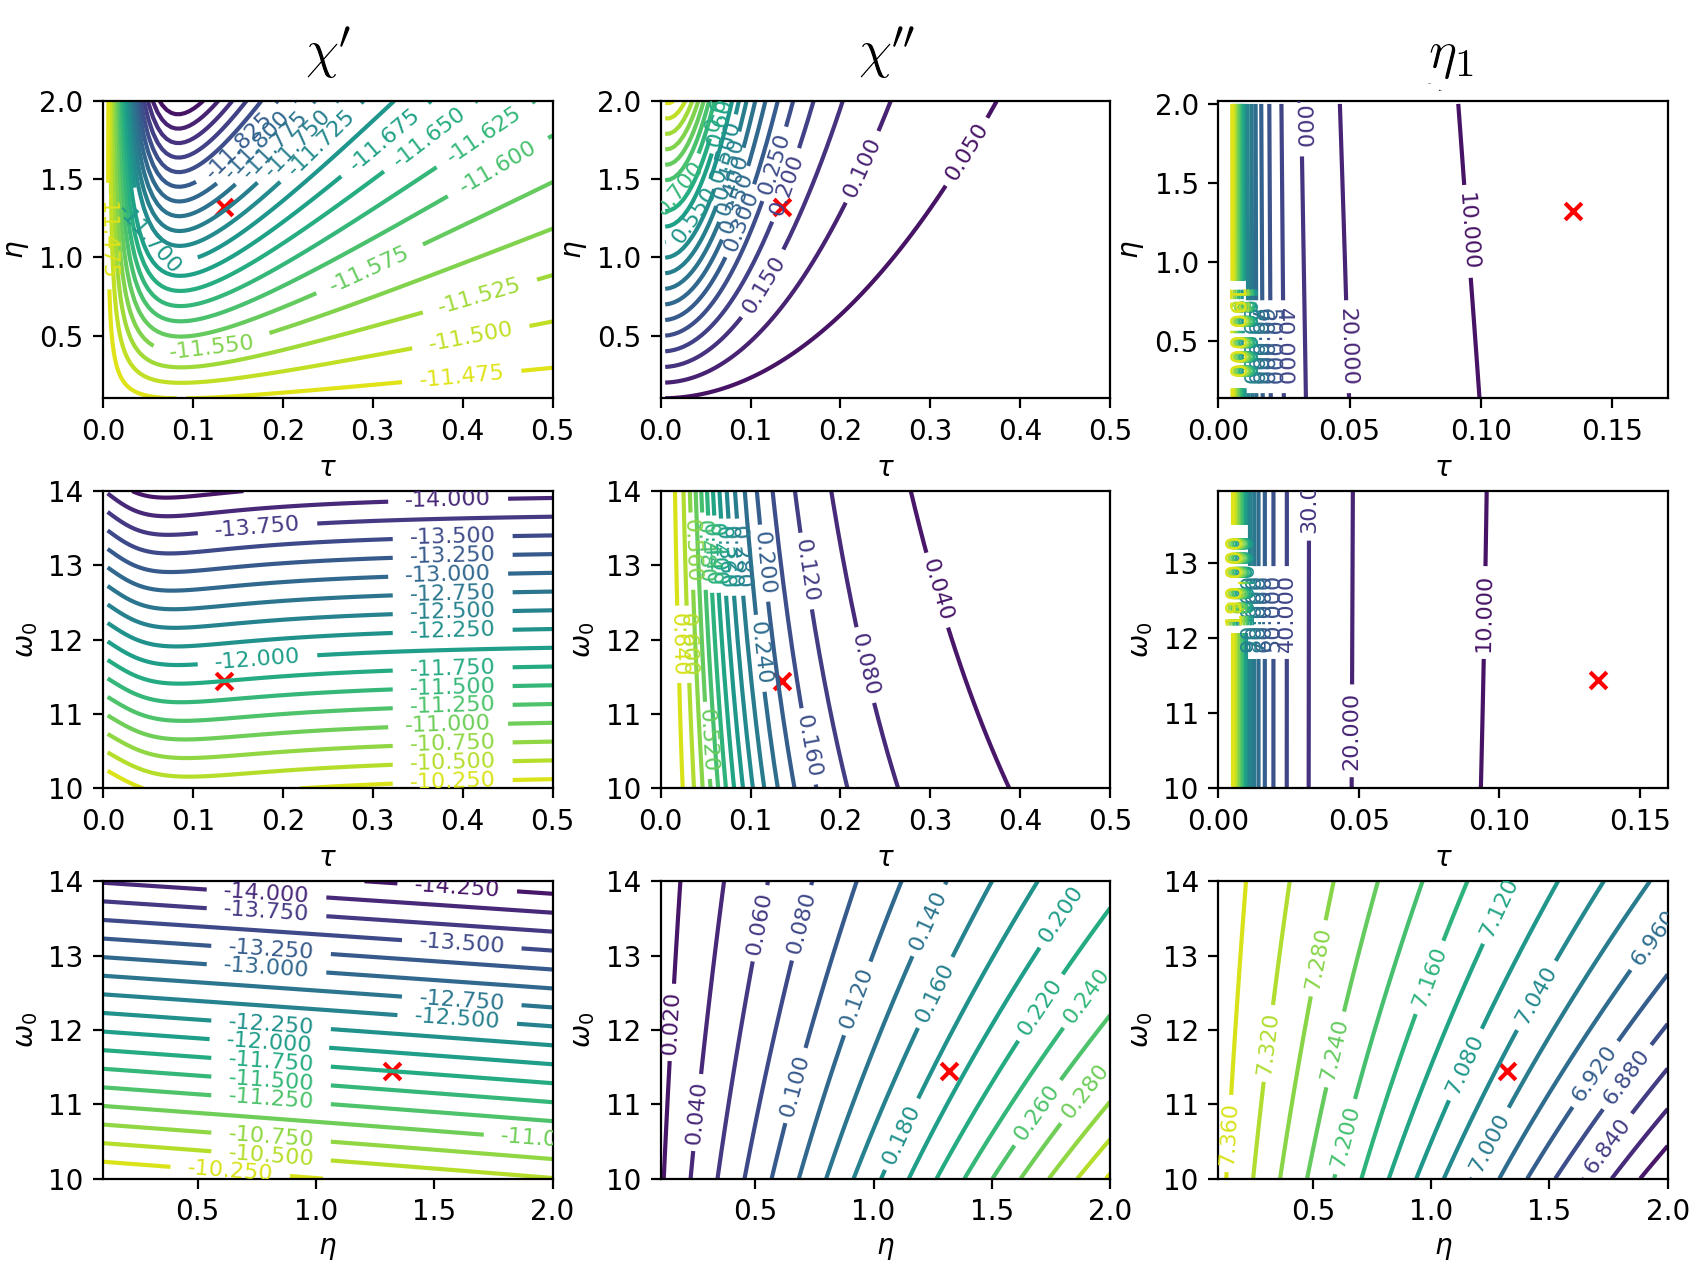
\includegraphics[width=1.2\textwidth]{harmonic_gle_parameters}}
		\caption{Contour plots showing the relationship between the position of the poles of the GLE Green's function and the GLE parameters $\omega_0$, $\eta$ and $\tau$. Each column contains contour plots for one of the pole parameters and the red crosses denote the value of GLE parameters typically encountered in this report.}
		\label{fig:pole_parameters}
	\end{subfigure}

	\begin{subfigure}{1.0\textwidth}
		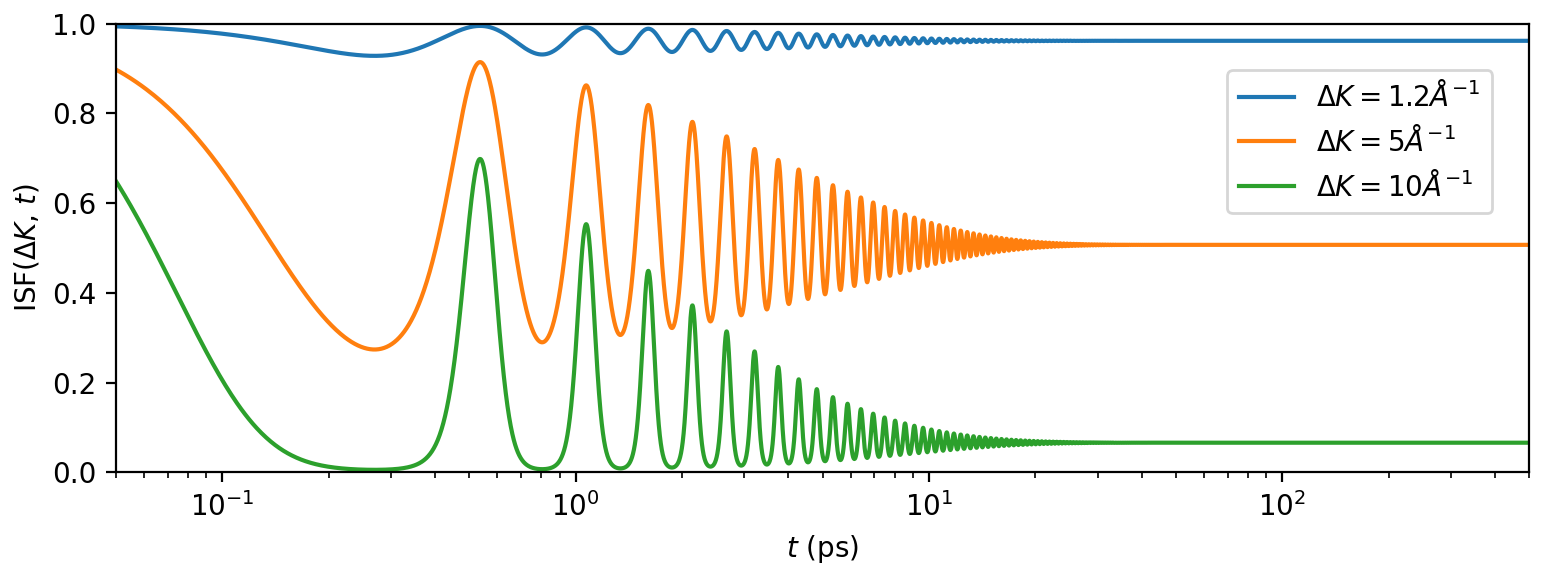
\includegraphics[width=1.0\textwidth]{analytic_isfs}
		\caption{ISFs of a particle in a harmonic potential well of natural frequency $\omega_0=\SI{11.45}{\ips}$ obeying the GLE with parameters $\tau=\SI{0.135}{\ps}$ and $\eta = \SI{1.34}{\ips}$ across a range of momentum transfers. Oscillations within the potential well are more pronounced at higher momentum transfers which suggests a means for extracting GLE parameters from experimental data at high momentum transfers.}
		\label{fig:analytic_isfs}
	\end{subfigure}

	\caption{}
\end{figure} 

\chapter{Simulation Setup and Validation} \label{ch:sim_setup} 

\section{3D Molecular Dynamics Simulation} \label{sec:md_setup}

\subsection{Construction of the Copper fcc Lattice Structure}

The construction of the MD simulation began by implementing the copper lattice model through a set of equilibrium lattice points. An fcc lattice was defined using the primitive basis vectors

\begin{align}
	\vec{b}_1 = a\left(1,1,0\right), \nonumber \\
	\vec{b}_2 = a\left(1,0,1\right), \label{eq:primitive_basis_vectors} \\
	\vec{b}_3 = a\left(0,1,1\right). \nonumber
\end{align}
\\
The lattice parameter $a=\SI{1.80}{\angstrom}$ was used, consistent with the lattice parameter of copper measured using x-ray crystallography \cite{davey}.
Harmonic nearest neighbor forces were implemented with force constant $k=\SI{28}{\newton\per\metre}$. This configuration has been shown to reproduce the phonon spectrum of copper \cite{sinha}. Periodic boundary conditions were imposed in the $\left[1,0,\bar{1}\right]$-$\left[0,1,\bar{1}\right]$ plane and the bottom layer of the substrate in the $\left[1,1,1\right]$ direction was was held fixed at its equilibrium position to prevent undesirable center of mass motion of the crystal. The top layer in the $\left[1,1,1\right]$ direction (which corresponds to a 111 surface for an fcc crystal) was left as a free surface on which a single adatom could be placed. The physical structure of the substrate is summarized in Figure \ref{fig:crystal_structure}.

\begin{figure}
	\begin{subfigure}[t]{0.45\textwidth}
		\centering
		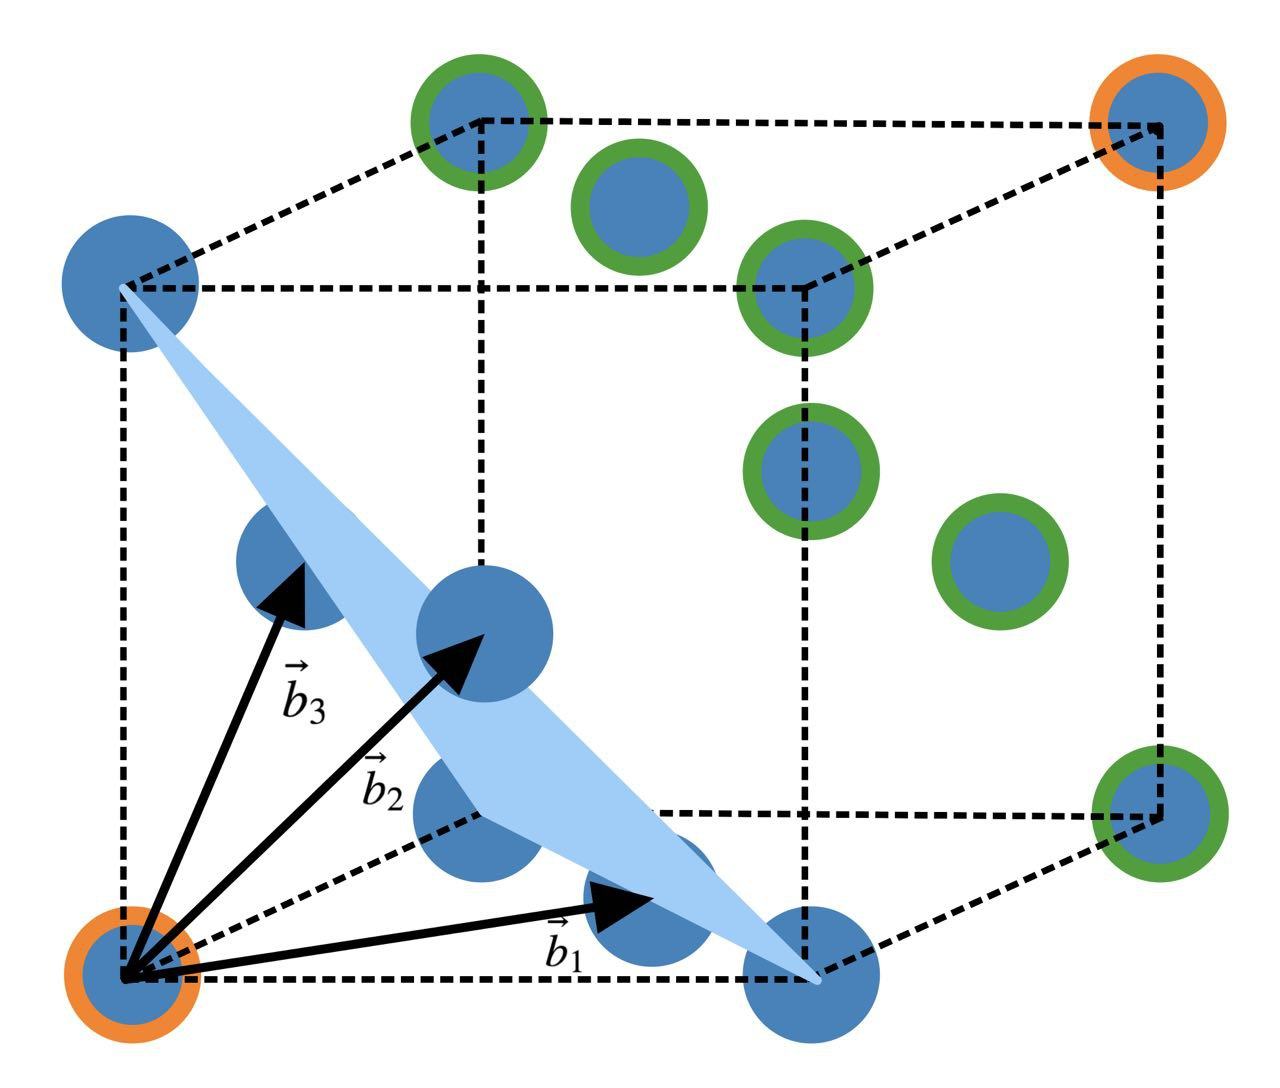
\includegraphics[width=1.0\textwidth]{fcc_cell}
		\caption{The form of the fcc crystal structure used in the simulation. Annotates the definitions of $\vec{b}_i$ in equation \ref{eq:primitive_basis_vectors} as well as the fcc 111 plane.} \label{fig:fcc_cell} 
	\end{subfigure}
	\hfill
	\begin{subfigure}[t]{0.45\textwidth}
		\centering
		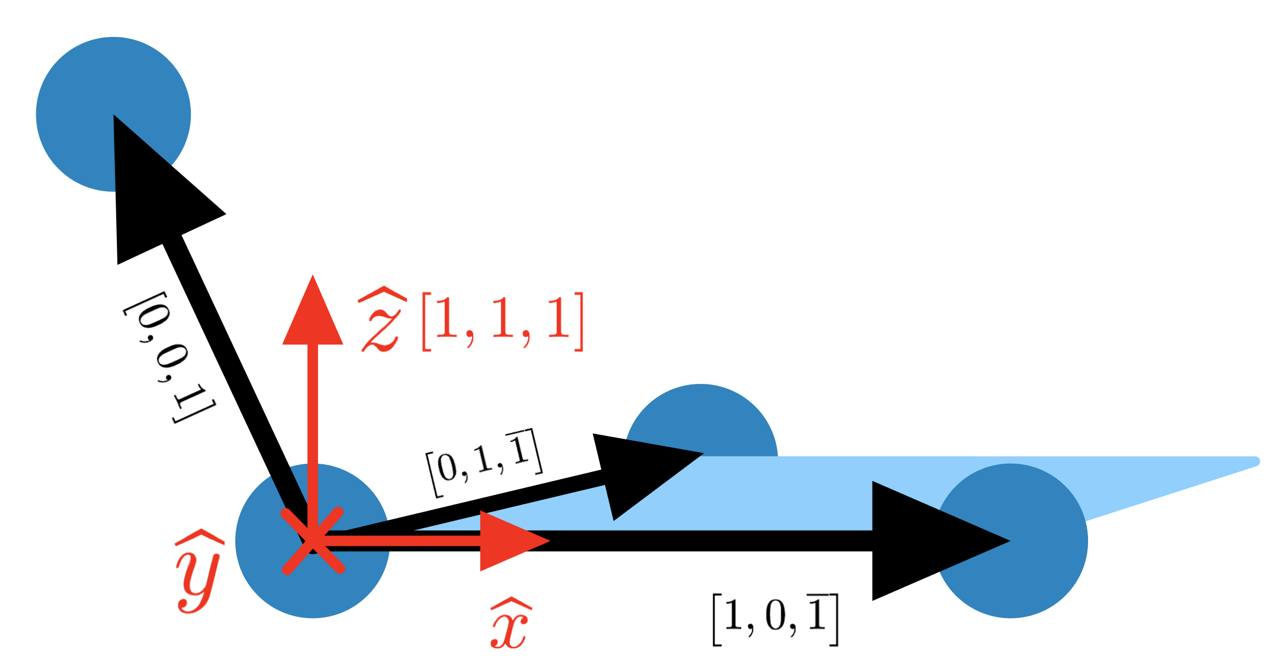
\includegraphics[width=1.0\textwidth]{in_plane_basis}
		\caption{Depicts the $\left[1,0,\bar{1}\right]$, $\left[0,1,\bar{1}\right]$ $\left[0,0,1\right]$ \& $\left[111\right]$ directions after rotating the crystal to align the 111-plane with the xy-plane.\label{fig:in_plane_basis}}
	\end{subfigure}
	\hfill
	\begin{subfigure}[t]{0.45\textwidth}
		\centering
		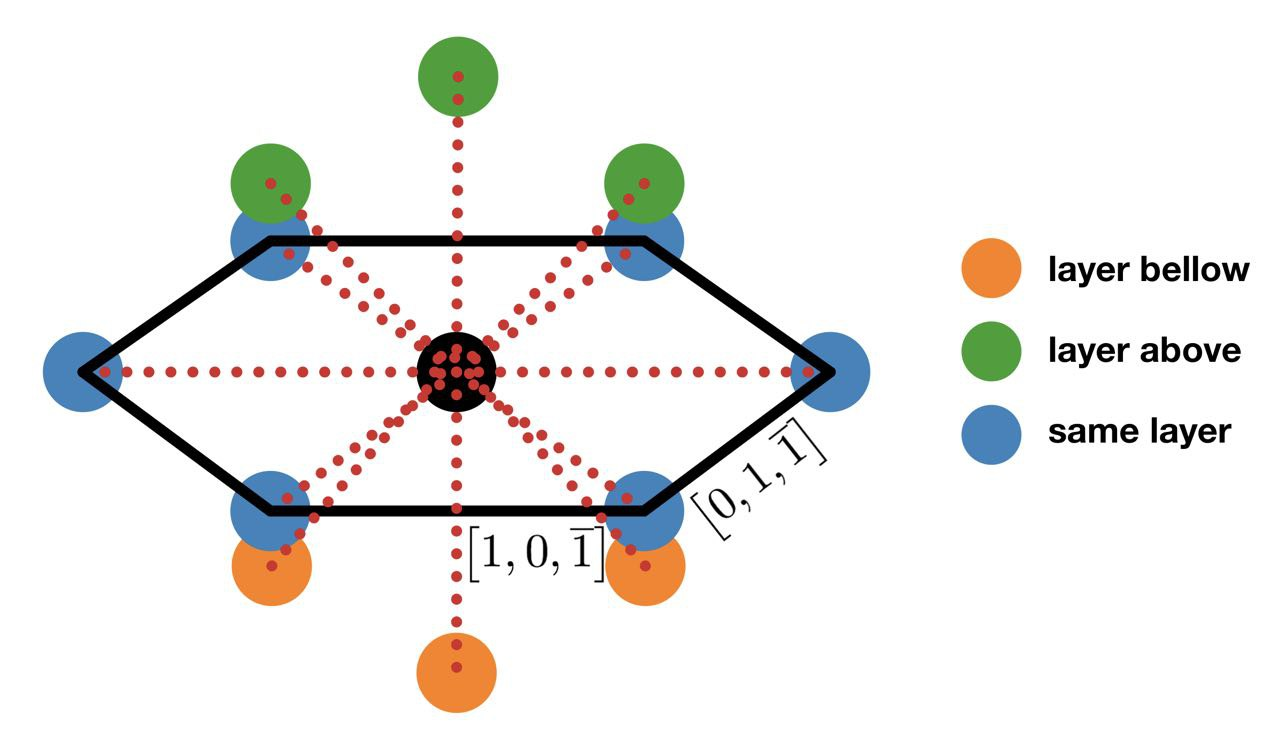
\includegraphics[width=1.0\textwidth]{nearest_neighbours}
		\caption{Each atom in the crystal is connected to its twelve nearest neighbors with a spring of natural length equal to the nearest neighbor distance of the fcc crystal ($2.54\angstrom$).} \label{fig:nearest_neighbours}	
	\end{subfigure}
	\hfill
	\begin{subfigure}[t]{0.45\textwidth}
		\centering
		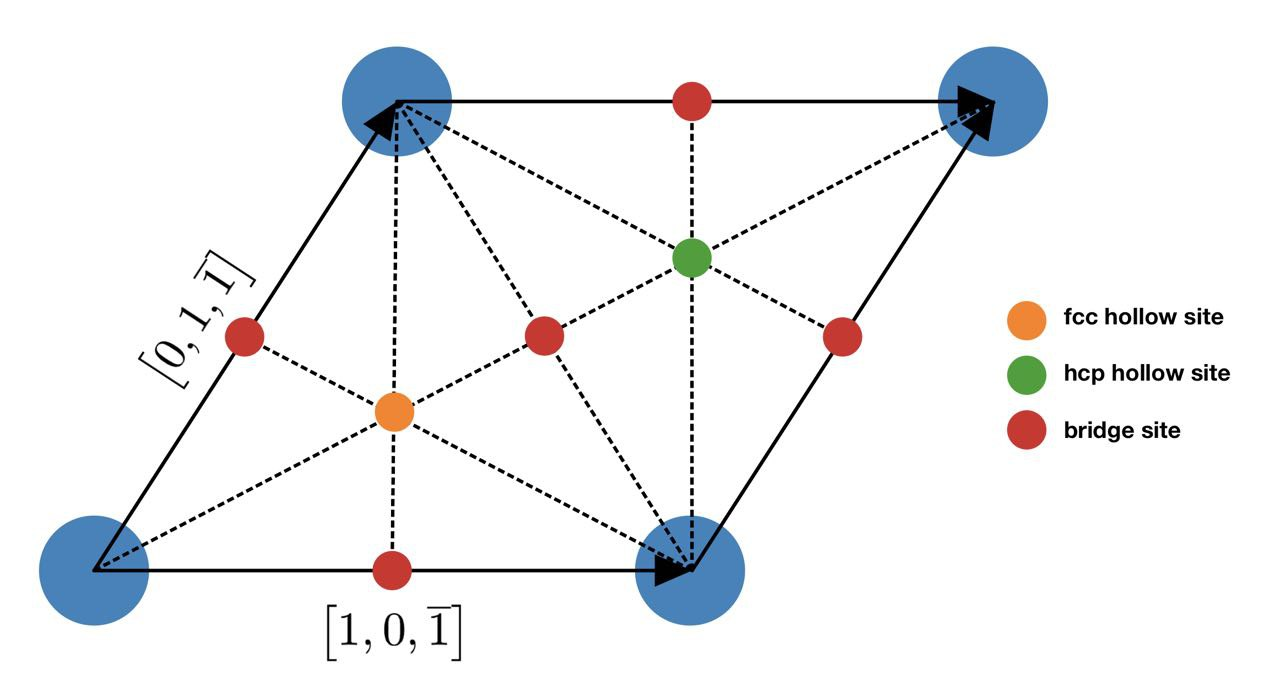
\includegraphics[width=1.0\textwidth]{primitive_cell}
		\caption{The top 111-plane in the crystal is tiled by the shown unit cell.} \label{fig:in_plane_cell}
	\end{subfigure}
\caption{Depiction of the fcc crystal structure with lattice parameter $1.8\angstrom$ used in the simulation to model a copper crystal with a free 111 plane.}
\label{fig:crystal_structure}
\end{figure}

\subsection{Adsorbate Substrate Interactions}

\begin{figure}
	\centering
	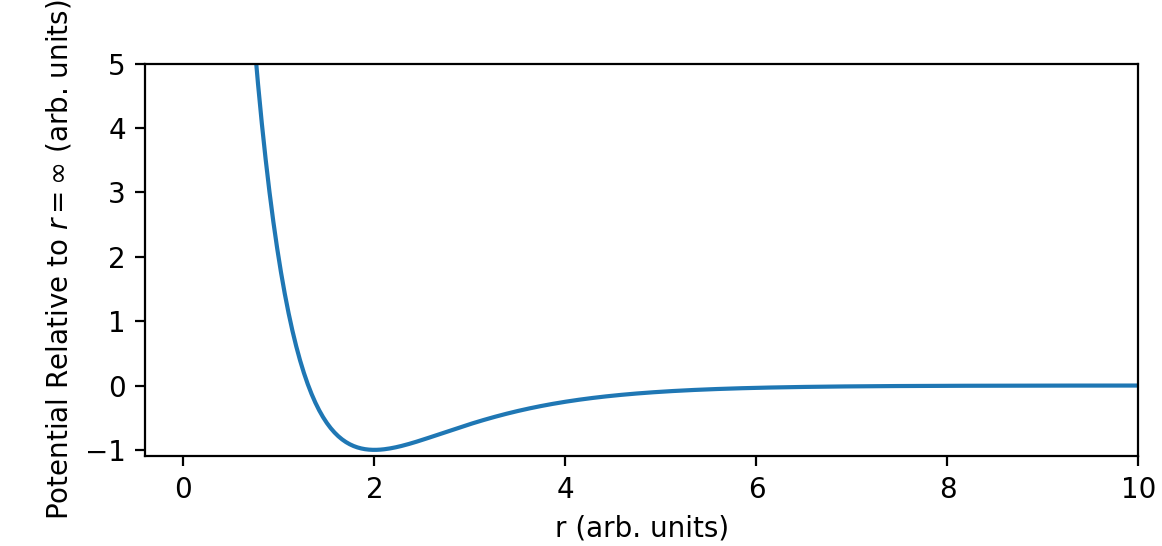
\includegraphics[width=0.8\textwidth]{morse_potential}
	\caption{The typical shape of a Morse potential as a function of particle separation.}
	\label{fig:morse_potential}
\end{figure}

A Morse potential (Figure \ref{fig:morse_potential}) was chosen for the adatom-substrate interaction given by the formula 
\begin{equation}
	V\left(r\right) = D(1-e^{-a\left(r-r_0\right)})^2 \label{eq:morse}
\end{equation}
where $D,a$ and $r_0$ are free parameters which control the depth, width and position of the potential well. This is a common choice for MD simulations \cite{SHUSTOROVICH19981, ELLIS199499}. For computational efficiency, at each simulation time-step, only substrate atoms within $4.5 \times r_0$ of the adatom (modulo the periodic boundary conditions) were included in the interaction. 

\subsection{Initializing and Propagating the Simulation}

In order to achieve the desired equilibrium temperature, the equipartition theorem requires the total amount of energy in the system equal $\frac{1}{2}N_{\text{dof}}k_BT$ \cite{Pathria}. The simulation was therefore initialized with all atoms at their equilibrium positions and the initial value of each velocity component sampled from a Gaussian with zero mean and variance $2 \cdot \frac{k_BT}{m}$. The center of mass velocity of the system was subtracted off to remove unwanted oscillations of the whole substrate off the fixed bottom layer.

At each time-step, the simulation was updated using a Velocity Verlet integrator. This method is commonly used in simulations in which the forces only depend on the positions of the particles involved \cite{Omelyan, Choi}. This gives a set of update equations
\\
$$
	\vec{x}_{n+1} = \vec{x}_n + \vec{v}_n \Delta{t} + \frac{1}{2m}\vec{F}\left(\vec{x}_n\right) \Delta{t}^2
$$
\begin{equation}
	\vec{v}_{n+1} = \vec{v}_n + \frac{1}{2m} \left(\vec{F}\left(\vec{x}_n\right) + \vec{F}\left(\vec{x}_{n+1}\right)\right) \Delta{t}
\end{equation}
\\
which were solved for each particle using a program written in Python 3.7. The operations were vectorized using the numpy library \cite{harris2020array} to ensure the program executed at reasonable speeds while written in Python. The simulation was found to be stable using a time-step of $\Delta{t}=\SI{10}{\femto\second}$, consistent with the result found in \cite{ELLIS199499}. 

\section{Validation of the 3D Molecular Dynamics Simulation}

\subsection{Oscillations near equilibrium}

The first check on the implementation of the MD simulation was performed by setting up a small piece of substrate with two atoms. One atom was held in place in the bottom layer and the other was allowed to oscillate freely. The oscillations of the free atom remained radial with an angular frequency consistent with a spring constant of $\SI{28}{\newton\per\metre}$.

A similar check was performed with an adatom and a single substrate atom which was held in place. The frequency of oscillation for small displacements was found to be consistent with the curvature of the Morse potential at the equilibrium position.

\subsection{Substrate Phonon Spectrum} \label{sec:phonon_spectrum}

\begin{figure}
	\centering
	\begin{subfigure}[t]{0.32\textwidth}
		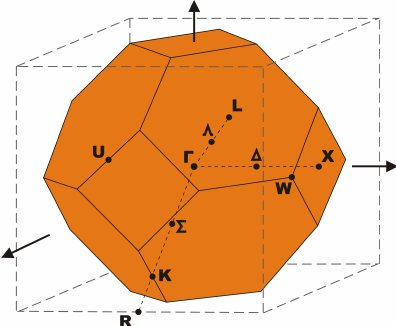
\includegraphics[width=1.0\textwidth]{fcc_brillouin_zone}
		\caption{The fcc Brillouin zone notation used in Figure \ref{fig:experimential_phonon_dispersion_plot} \& \ref{fig:phonon_dispersion_plot} \cite{Zaleski}.}
		\label{fig:fcc_notation}
	\end{subfigure}
	\hfill
	\begin{subfigure}[t]{0.63\textwidth}
		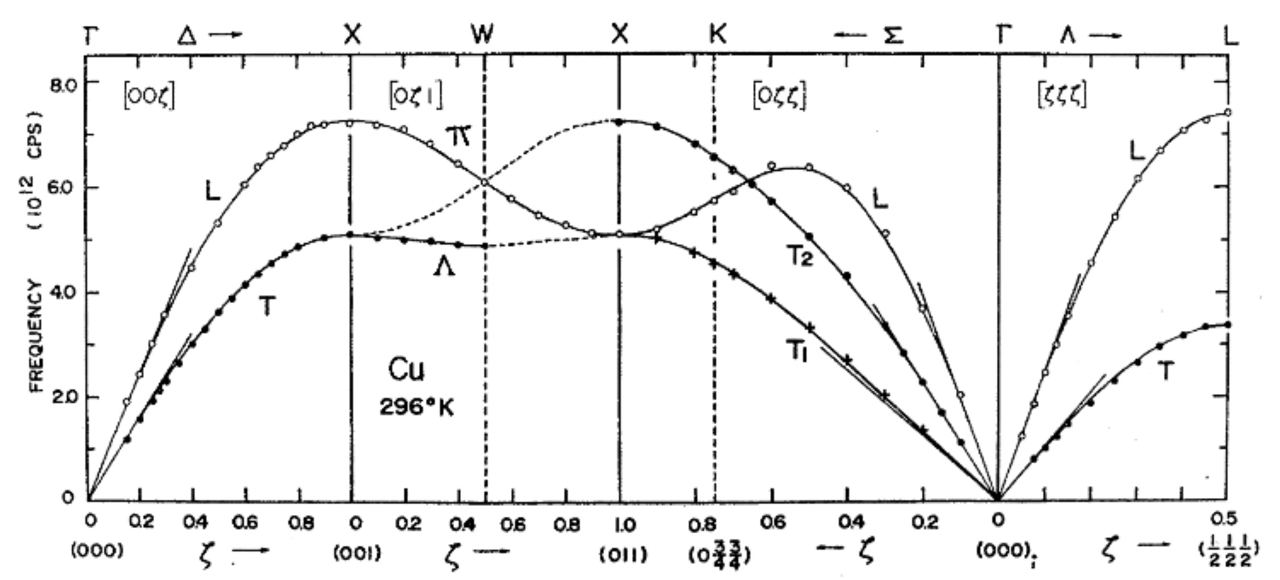
\includegraphics[width=1.0\textwidth]{copper_bulk_phonon_dispersion_curve}
		\caption{The phonon dispersion curves of copper extracted from neutron scattering data at $\SI{296}{\kelvin}$ \cite{Svensson}.}
		\label{fig:experimential_phonon_dispersion_plot}
	\end{subfigure}
	\begin{subfigure}[t]{1.0\textwidth}
		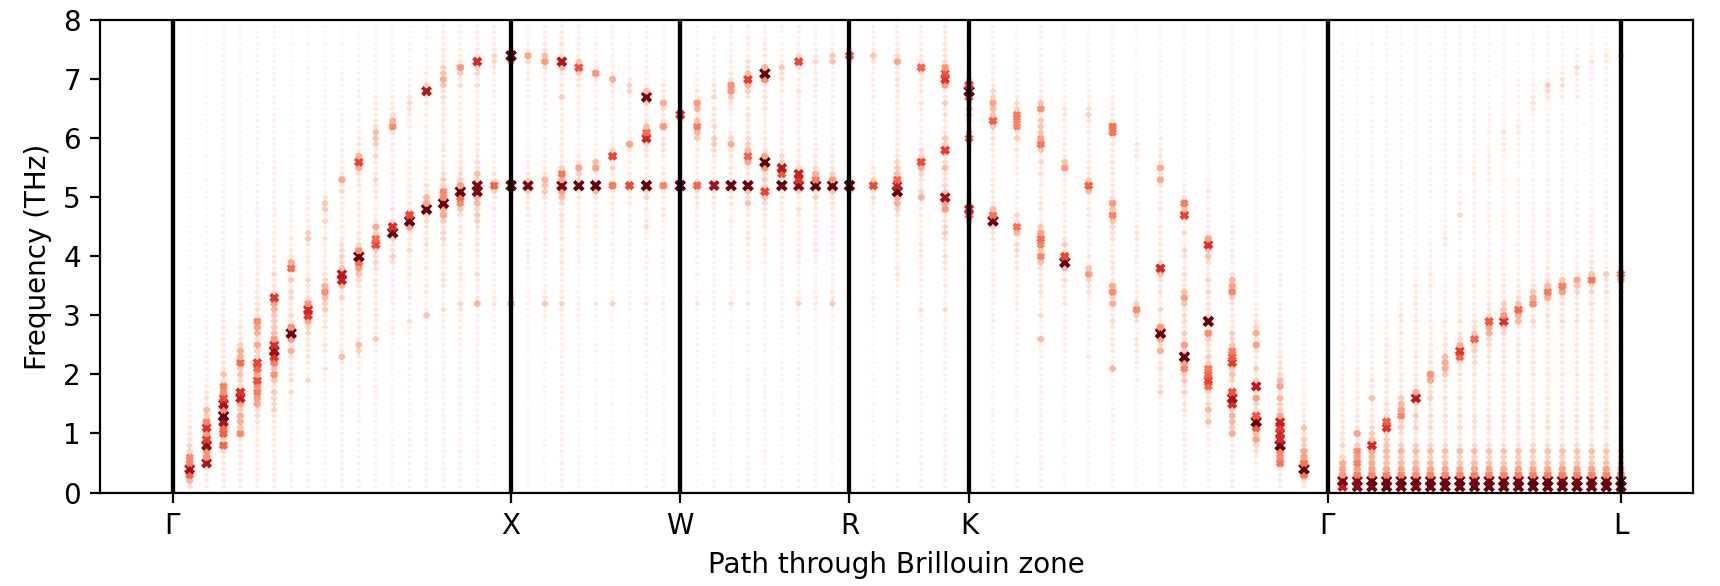
\includegraphics[width=1.0\textwidth]{phonon_dispersion_plot}
		\caption{A substrate phonon dispersion plot extracted from the simulation at $\SI{296}{\kelvin}$ with no adatoms present. Substrate distortions due to the pinned bottom layer are visible in the $\Gamma\rightarrow \mathrm{L}$ direction.}
		\label{fig:phonon_dispersion_plot}
	\end{subfigure}
	\caption{}
	\label{fig:phonons}
\end{figure}

The implementation of the substrate's structure and periodicity was validated by comparing the phonon spectrum observed in the simulated lattice to the known phonon spectrum in copper shown in Figure \ref{fig:experimential_phonon_dispersion_plot} \cite{sinha}. 

The simulation was run with a $40\times40\times40$ substrate and no adatoms present for $\SI{100}{\pico\second}$ at $\SI{296}{\kelvin}$. A sequence of k-vectors was defined using a path through the fcc Brillouin zone to match Figure \ref{fig:experimential_phonon_dispersion_plot} as per the fcc Brillouin zone notations in Figure \ref{fig:fcc_notation}. Using this sequence of k-vectors, Figure \ref{fig:phonon_dispersion_plot} was produced using the last $\SI{10}{\pico\second}$ of the run and the formula
\begin{equation}
	A_{\text{phonon}}\left(\vec{k}, f\right) = \int dt \exp\left(-2\pi i ft\right) \sum_{n,k,l=1}^{N,K,L}\sum_{i=1}^3\exp\left(-\vec{k}\cdot\vec{r}_{n,k,l}\right)\left(\vec{\epsilon}_i\cdot\Delta\vec{r}_{n,k,l}\left(t\right)\right)
\end{equation}
\\
where $\vec{k}$ and $f$ are the wave-vector and frequency of a candidate phonon, $\vec{\epsilon}_i$ are three unit vectors spanning the phonon's polarization space, $\vec{r}_{n,k,l}$ is the equilibrium position of the atom with index $n,k,l$ and $\Delta\vec{r}_{n,k,l}$ is its displacement vector. The large red crosses in Figure \ref{fig:phonon_dispersion_plot} correspond to stable modes of oscillation of the crystal and therefore illuminate the substrate's phonon dispersion curves. These curves demonstrate that the simulation reproduces the physical phonon spectrum of copper in Figure \ref{fig:experimential_phonon_dispersion_plot}. Distortions are clearly visible in the $\Gamma\rightarrow\mathrm{L}$ (corresponding to $\left[111\right]$) direction due to the fixed bottom layer and lack of periodicity in this direction. 

\subsection{Thermodynamic Quantities}


\begin{figure}
	\centering
	\begin{subfigure}[t]{0.48\textwidth}
		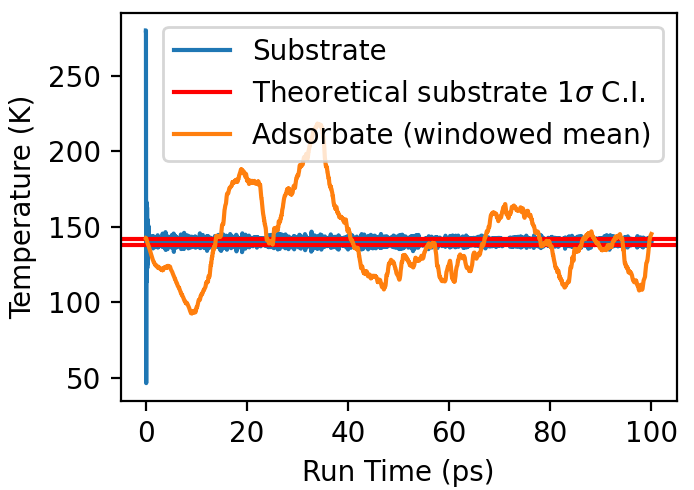
\includegraphics[width=1.0\textwidth]{md_temperature}
		\caption{Temperature as a function of time for the run. The theoretical $\mu \pm 1\bar{\sigma}$ confidence interval accounting for fluctuations of the substrate's kinetic energy is shown in red ($\bar{\sigma}=\sqrt{\frac{5}{3N}}T$).}
		\label{fig:md_temperature}
	\end{subfigure}
	\hfill
	\begin{subfigure}[t]{0.48\textwidth}
		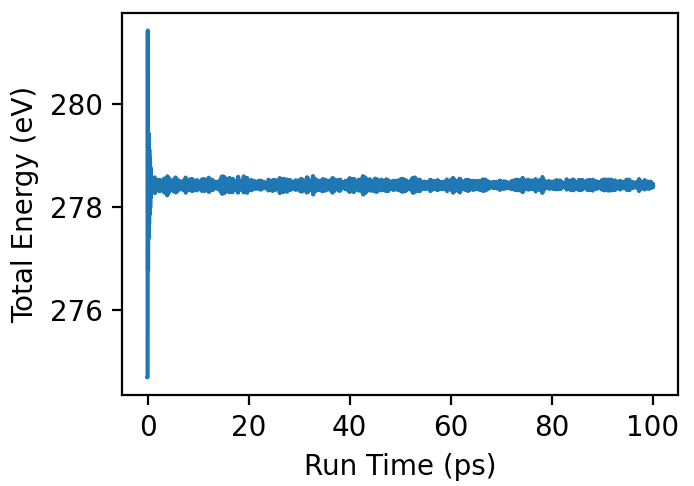
\includegraphics[width=1.0\textwidth]{md_total_energy}
		\caption{Total energy as a function of time. The system is observed to quickly equilibriate with small but bound fluctuations around the equilibrium value due to numerical error.}
		\label{fig:md_total_energy}
	\end{subfigure}
	\begin{subfigure}[t]{0.9\textwidth}
		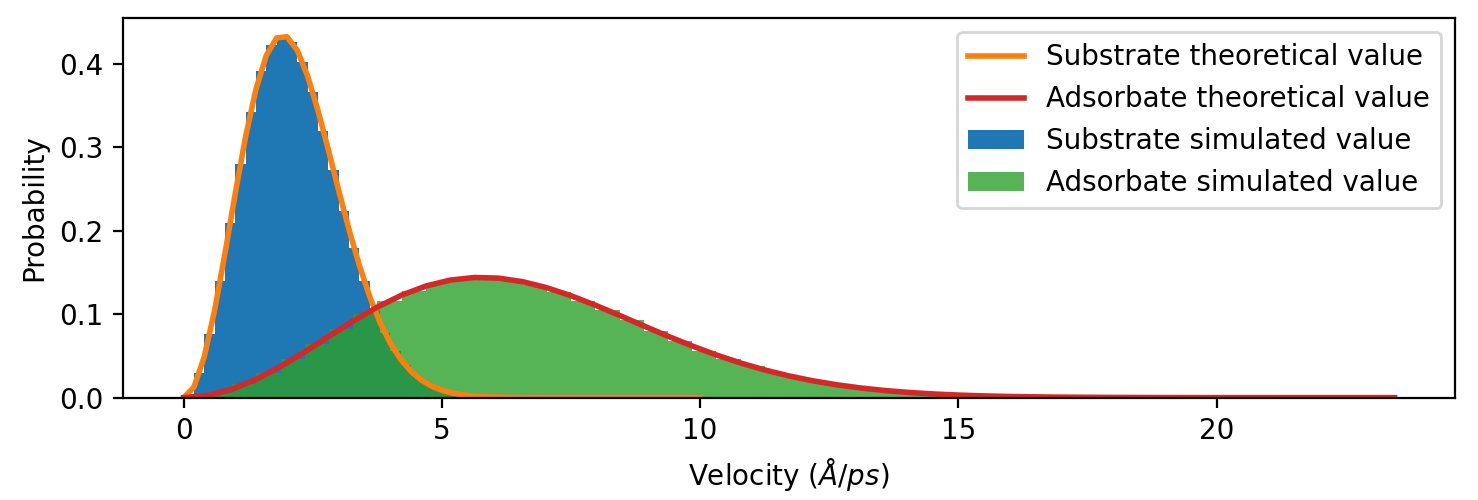
\includegraphics[width=1.0\textwidth]{md_velocities}
		\caption{Histograms of the speed of the adatom and substrate particles super-imposed with their respective theoretical 3D Maxwell-Boltzmann distributions.}
		\label{fig:md_velocities}
	\end{subfigure}
	\caption{Example plots of the thermodynamic quantities monitored in each simulation run. The shown run was performed at $\SI{140}{\kelvin}$ for $\SI{100}{\pico\second}$.}
	\label{fig:thermodynamics}
\end{figure}

The temperature, total energy and speed distribution of each simulation run were carefully monitored to ensure that they agreed with their theoretical values. The temperature of the substrate was calculated using the equipartition theorem, $T=\frac{2}{3k_B}\left<E_k\right>$ where $\left<E_k\right>$ is the average kinetic energy of the substrate atoms. Figure \ref{fig:thermodynamics} shows a typical set of these thermodynamic quantities. All runs reported were found to equilibriate within $\SI{1}{\pico\second}$ and fluctuate around equilibrium within the expected theoretical bounds. All analysis either excluded the first few picoseconds of a run or the simulation was run long enough for the equilibriation period to be considered negligible.

\section{Fitting Simulation Parameters to Features of Lithium on Copper(111)} \label{sec:md_fit}

\begin{table}[h!]
	\centering
\begin{tabular}{ |p{3.5cm}|p{2.2cm}|p{1.8cm}||p{2.8cm}|p{2.8cm}|}
 \hline
 \multicolumn{5}{|c|}{Results of Parameter Optimization} \\
 \hline
	Feature & Target Value & Fit Value & Morse Parameter & Optimized Value \\
 \hline
	$\left[111\right]$ Vibration Freq. & $\SI{38}{\milli\eV}$ \cite{livibfreq} & $\SI{36.2}{\milli\eV}$ & $D$ & $\SI{103.7}{\mev}$ \\
	Equilibrium Height & $\SI{2.1}{\angstrom}$ \cite{PADILLACAMPOS1997183} & $\SI{2.2}{\angstrom}$ & $a$ & $\SI{1.527}{\angstrom}^{-1}$ \\
	fcc/hcp Pot. Diff. & $\SI{0}{\mev}$ \cite{Guido,Ward} & $\SI{0.4}{\mev}$ & $r_0$ & $\SI{2.896}{\angstrom}$ \\
	Bridge Site Barrier & $\SI{9}{\mev}$ \cite{PADILLACAMPOS1997183, Ward} & $\SI{9.4}{\mev}$ & & \\
 \hline
\end{tabular}
	\caption{The features of lithium on copper used to fit the Morse parameters in equation \ref{eq:morse}. The fitting routine was setup to produce properties close in value to those estimated by independent sources. The best fit parameters and their resulting simulated features are also shown.} 
\label{table:fit_parameters}
\end{table}

Having constructed and validated the 3D molecular dynamics simulation, a fitting routine was constructed to optimize the Morse parameters in the simulation to fit various properties of lithium on copper. Given a set of Morse parameters, a routine was setup to determine the equilibrium height and vibration frequency of an adatom in the $\left[111\right]$ direction as well as the potential difference between the two hollow sites in the fcc crystal and the barrier height between them. These properties have been independently estimated for lithium on copper and are summarized in Table \ref{table:fit_parameters}. 

The $\left[111\right]$ vibration frequency was determined by confining the motion of the adatom above a hollow site to the $\left[111\right]$ direction and allowing the adatom to oscillate in place. The vibration frequency was then extracted from the peak in the Fourier spectrum of the atom's $\left[111\right]$ coordinate.

The equilibrium height and potential for each hollow/bridge site was determined by similarly pinning the adatom's position over a site and running the simulation for a short time while damping the motion of the system. Once the system had relaxed, the equilibrium height relative to the substrate was read off and the potential energy of the configuration was calculated as the sum of the energy stored in the Morse interactions as well as the energy in the substrate's inter-atomic bonds due to lattice deformations.

Using the target values in Table \ref{table:fit_parameters} a simple weighted squared difference cost function was implemented and a scipy.optimize.minimize \cite{2020SciPy-NMeth} optimizer instance was used to find a set of Morse parameters which minimize the cost function. The outcome of this fitting process is included in Table \ref{table:fit_parameters}. It was found that the Morse $D$ parameter was largely untouched by the optimizer regardless of its initial value. Therefore future work may be able to fit additional properties using this degree of freedom.

\subsection{Extraction of the Potential Energy Surface} \label{sec:extract_potential}


\begin{figure}
	\centering
	\begin{subfigure}[t]{0.48\textwidth}
		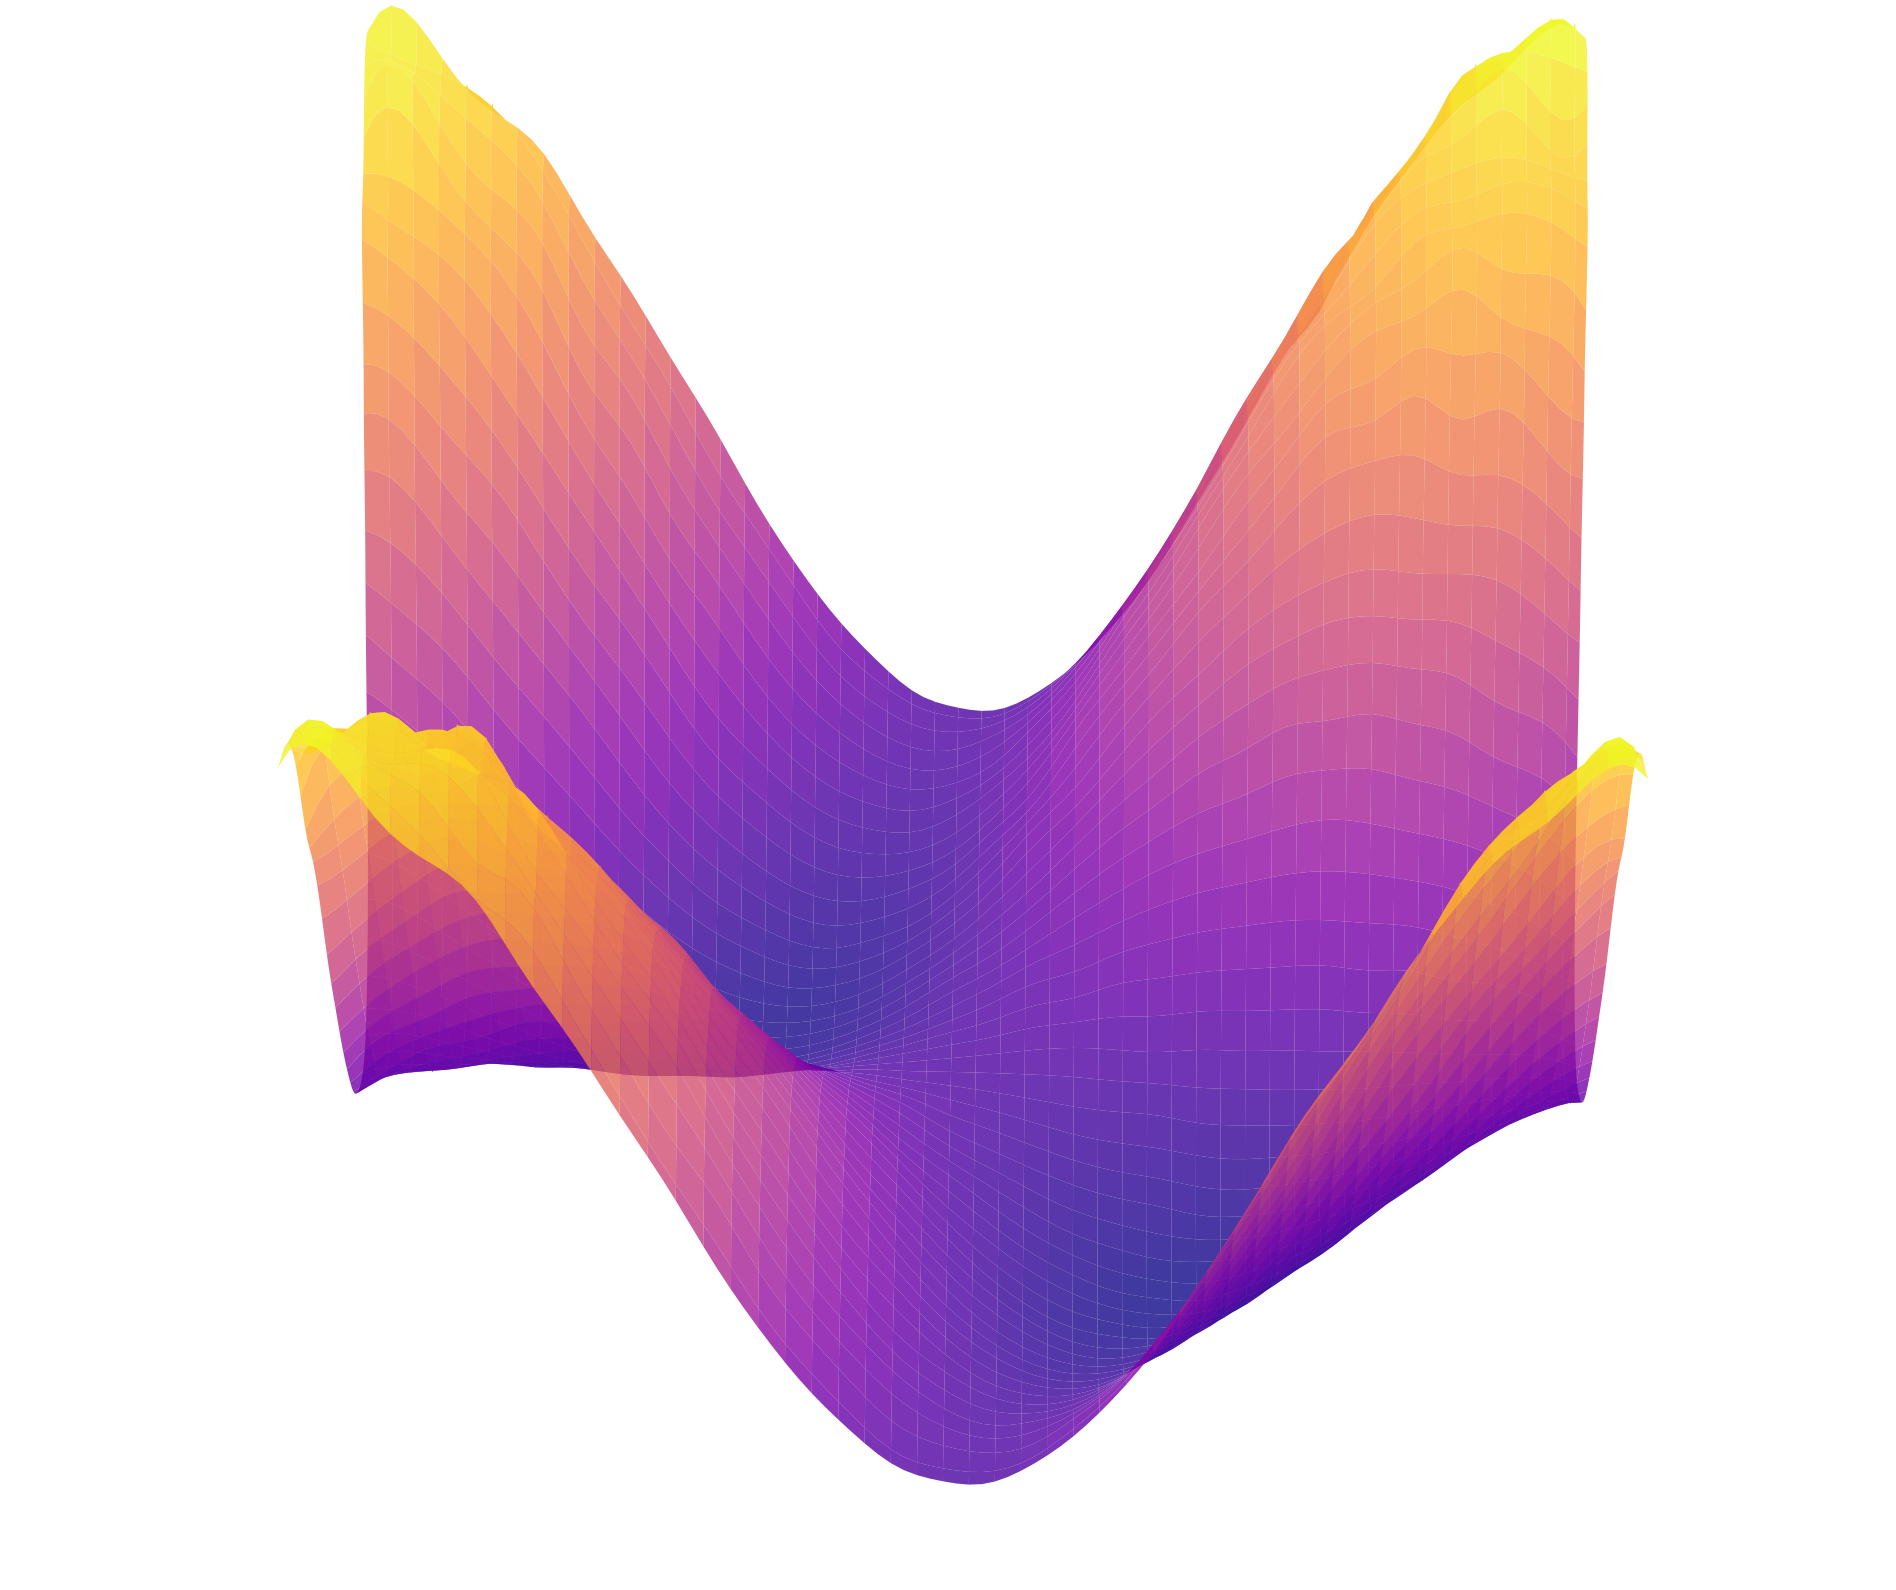
\includegraphics[width=1.0\textwidth]{potential_surface}
		\caption{The 2D potential surface seen by an adatom in the 3D molecular dynamics simulation. Obtained by inverting the Boltzmann factor $P(\vec{x}) \propto e^{-V(\vec{x})/k_BT}$.}
		\label{fig:potential_surface_plot}
	\end{subfigure}
	\hfill
	\begin{subfigure}[t]{0.48\textwidth}
		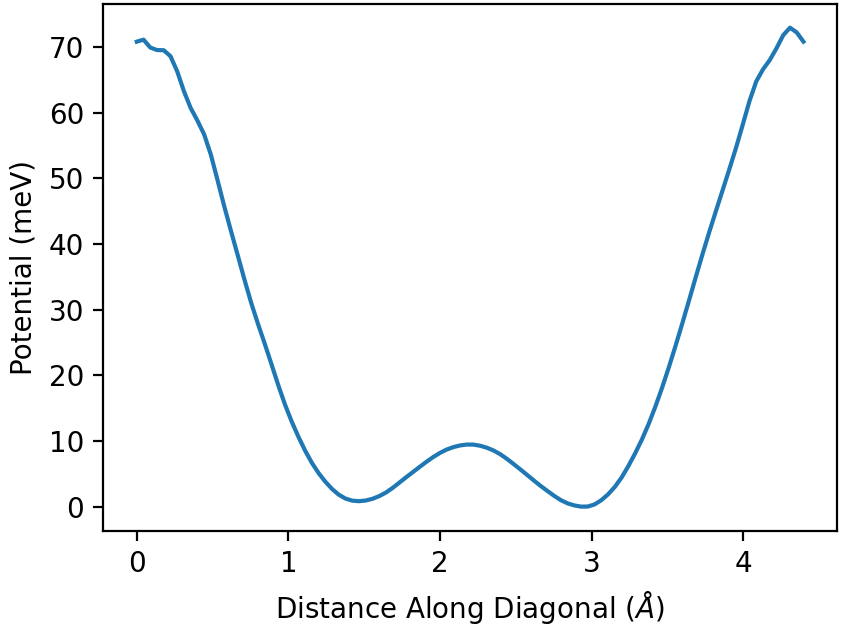
\includegraphics[width=1.0\textwidth]{potential_cross_section}
		\caption{A cross section of the potential surface through the diagonal of Figure \ref{fig:potential_surface_plot}. This exhibits a $\SI{9.4}{\mev}$ barrier height and a $\SI{0.4}{\mev}$ fcc/hcp hollow site potential difference.}
		\label{fig:potential_cross_section}
	\end{subfigure}
	\caption{}
	\label{fig:potential_surface}
\end{figure}

The equivalent 2D potential energy surface seen by the adatom in the 3D molecular dynamics simulation was extracted by running the simulation for $\SI{100}{\nano\second}$ with the a $20\times20\times20$ substrate using the parameters in Table \ref{table:fit_parameters}. Each point in the simulated trajectory was mapped back to its equivalent position within the first 2D unit cell on the surface (see Figure \ref{fig:in_plane_cell}). These points were binned on a $30\times30$ grid to provided an estimate of the probability of finding the adatom in each bin at any given time\footnote{Any bins which saw no occupation were assigned an occupation probability of one hundredth of the lowest non-zero occupation probability.}. This probability is proportional to a Boltzmann factor, $P\left(\vec{x}\right) \propto e^{-V\left(\vec{x}\right)/k_BT}$ \cite{Pathria}. This relationship was inverted and the resulting potential surface is shown in Figure \ref{fig:potential_surface}. The statistical noise present on the corners (corresponding to lattice points) was safely ignored since the adatom will very rarely find itself close to these points.

\section{Implementation of the Generalized Langevin Equation Simulations}

A Generalized Langevin Simulation as described in Section \ref{sec:gle_with_background} was constructed using the potential surface extracted from the 3D molecular dynamics simulation shown in Figure \ref{fig:potential_surface}. The $30\times30$ potential grid was interpolated using a scipy.interpolate.RectBivariateSpline \cite{2020SciPy-NMeth} instance and the force at a given position was calculated from the gradient of the potential. 

An exponential memory kernel of the form $K\left(t\right) = \theta(t)\frac{1}{\tau}\exp\left(-\frac{t}{\tau}\right)$ was chosen for its ease of implementation and low computational cost. The discrete memory kernel convolution was implemented using the relation
\\
$$
\int_0^{t_n} dt' K\left(t-t'\right) \vec{f}(t') \approx \alpha \int_0^{t_{n-1}} dt' K\left(t-t'\right) \vec{f}(t') + \frac{1}{1-\alpha} \vec{f}\left(t_n\right)
$$
\\
where $\alpha = \exp{\frac{-\Delta{t}}{\tau}}$ and $\Delta{t}$ is the simulation time-step ($\SI{1}{\femto\second}$ in this case). The normalization factor $\frac{1}{1-\alpha}$ ensures that the total impulse imparted by $\vec{f}(t_n)$ is unaffected by the discretization process. 

The GLE simulations were propagated through time using a Velocity Verlet integrator. Velocity Verlet integration is frequently used in Langevin type simulations \cite{Ward, Townsend}. However, the velocity dependent friction force and non-analytic stochastic force present in Langevin type equations brings into question this choice of integrator \cite{gronbech2013simple}. The performance of the Velocity Verlet integrator and a `modified' Velocity Verlet integrator \cite{Omelyan} are evaluated in the presence of a background potential in Section \ref{sec:thermalization}.

The GLE simulation was tested using a harmonic potential and compared to the theoretical results derived in \ref{sec:gle_interpretation}. The simulation ISF and analytical expressions were found to match exactly. 


\chapter{3D Molecular Dynamics Results and Comparison with Experimental Data}

The 3D molecular dynamics simulation was run for $\SI{100}{\nano\second}$ at $\SI{140}{\kelvin}$ using the Morse parameters in Table \ref{table:fit_parameters} and a $20\times20\times20$ substrate. The results of this simulation are summarized in Figure \ref{fig:md_results}.

\section{Discussion and Analysis of ISFs}

Figures \ref{fig:md_isf_0.6} \& \ref{fig:md_isf_1.2} show the simulated ISFs in the $\left[11\bar{2}\right]$ direction overlayed with experimental HSEM data\footnote{The experimental data is shown as black crosses. The red, green and blue lines were included in the results in \cite{Ward} but may be ignored for the purposes of this report.\label{rgb_lines}} taken from \cite{Ward}. At very short times, $t \sim \SI{e-1}{\pico\second}$, we see agreement of the experimental data and the MD simulation. The Gaussian shape of the ISF at this very short timescale is driven by ballistic motion solely parameterized by the 2D thermal velocity of the lithium, $v=\sqrt{\frac{2k_BT}{m}}$ \cite{Ward}. Experimental results have shown that the effective mass of lithium on copper is equal to its atomic mass so this result is expected \cite{Ward}. 

At long times, the simulated ISFs are found to decay much faster than the experimental ones. Since the simulation was setup with a hopping potential barrier similar to the experimentally determined value, this classical simulation fails to capture the pre-exponential factor of the real system. 

The molecular dynamics simulation disagrees with experimental data on the relative contributions of fast to slow motion in the ISF. This is apparent in the proportion of the ISF's drop off which occurs in the first few picoseconds relative to the slow decay. Previous work on lithium on copper(111) has explained similar discrepancies by introducing GLE simulations with a band limited noise spectrum \cite{Ward}. However, the frequency cutoff required was found to be almost an order of magnitude lower than the phonon cutoff frequency in copper. This explains why the MD simulation, is unable to reproduce this aspect of the experimental data.

Figure \ref{fig:isf_0.6_dkz_included} is indicative of the additional structure in the ISF which is missed by the Cambridge HSEM apparatus due to insensitivity to the very high frequency components of the signal. In light of the discussion in Chapter \ref{sec:gle_interpretation}, these oscillations may be used to extract useful information about the system in the $\left[111\right]$ direction if they ever become experimentally accessible.

\section{Discussion and Analysis of simulated hopping rates}

Figure \ref{fig:alpha_deltak} shows the dephasing rate of the ISF in the $\left[1\bar{1}0\right]$ direction as a function of $\Delta{\vec{K}}$. As pointed out in \cite{TUDDENHAM20101459}, although the fcc 111 surface is not a Bravais lattice and the hops occur between between non-equivalent lattice sites, the ISF in the $\left[1\bar{1}0\right]$ direction is equivalent to a particle hopping on a 1D lattice with half the lattice spacing of the fcc crystal. The ISF of such idealized hopping is given by the Chudley-Elliot model and predicts a dephasing rate of
\\
$$
	\alpha\left(\Delta{K}\right) = 2\Gamma\sin^2\left(\frac{a\Delta{K}}{2}\right)
$$
\\
Where $\alpha$ is the dephasing rate, $\Gamma$ is the hopping rate and $a$ is the equivalent 1D nearest neighbor distance. Figure \ref{fig:alpha_deltak} therefore suggests that the simulation exhibits a hopping rate of $\SI{0.62}{\per\pico\second}$ for hops with a component in the $\left[1\bar{1}0\right]$ direction. Rotational symmetry of the system may then be used to argue that the total hopping rate is approximately $\Gamma_{\text{tot}} = \frac{3}{2}\Gamma = \SI{0.93}{\per\pico\second}$. Therefore the hopping of the system is likely to be sensitive to changes in the Fourier spectrum around $\sim\SI{1}{\tera\hertz}$ or less. Much higher frequencies noise components are unlikely to affect hopping as they average out over the timescale of a picosecond. 

Figure \ref{fig:ahrrenius_plot} Shows the logarithm of the maximum ISF dephasing rate as a function of inverse temperature. The fitting process used to extract the maximum dephasing rate was hindered by phonon oscillations and noise. This introduced a large degree of uncertainty into this estimate even when the Fourier filter method suggested in the \cite{Ward} was used. Nevertheless this results in \ref{fig:ahrrenius_plot} are consistent with an Arrhenius law with activation energy $E_a=9.6\pm\SI{1.5}{\mev}$ and confirm that the pre-exponential factor of the decay rate is not reproduced by MD simulation.

\begin{figure}
	\begin{subfigure}{0.49\textwidth}
		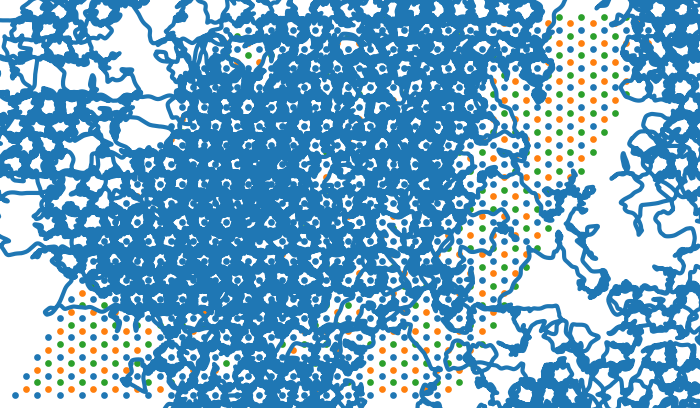
\includegraphics[width=1.0\textwidth]{md_top_down}
		\caption{The trajectory of the adatom overlayed on the equilibrium position of the top 3 substrate layers. Periodic substrate boundary conditions allow the adatom to diffuse outside the bounds of the substrate.}
		\label{fig:md_top_down}
	\end{subfigure}
	\hfill
	\begin{subfigure}{0.49\textwidth}
		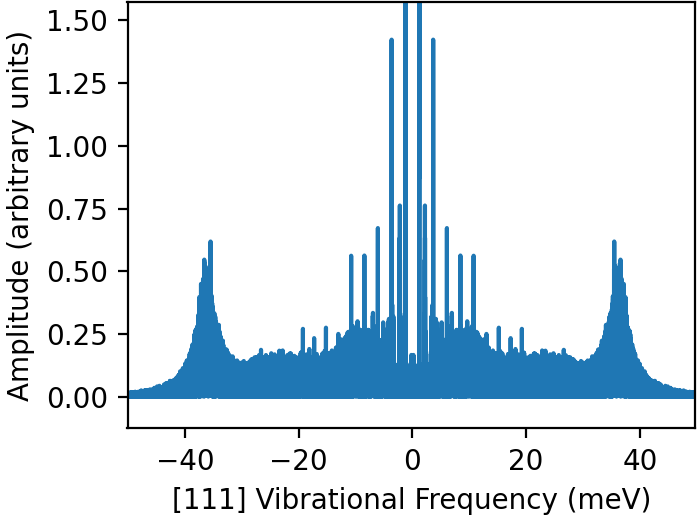
\includegraphics[width=1.0\textwidth]{111_vibrational_fft}
		\caption{The Fourier spectrum of the [111] co-ordinate of the adatom. The peak at $\SI{38}{\mev}$ corresponds to harmonic oscillations around equilibrium as constructed in Section \ref{sec:md_fit}. The phonon cutoff frequency determined in Section \ref{sec:phonon_spectrum} of $\SI{7.4}{\tera\hertz}$ ($\SI{30.5}{\mev}$) is visible but overlaps with the harmonic peak.}
		\label{fig:111_vibrational_fft}
	\end{subfigure}
	
	\begin{subfigure}{0.49\textwidth}
		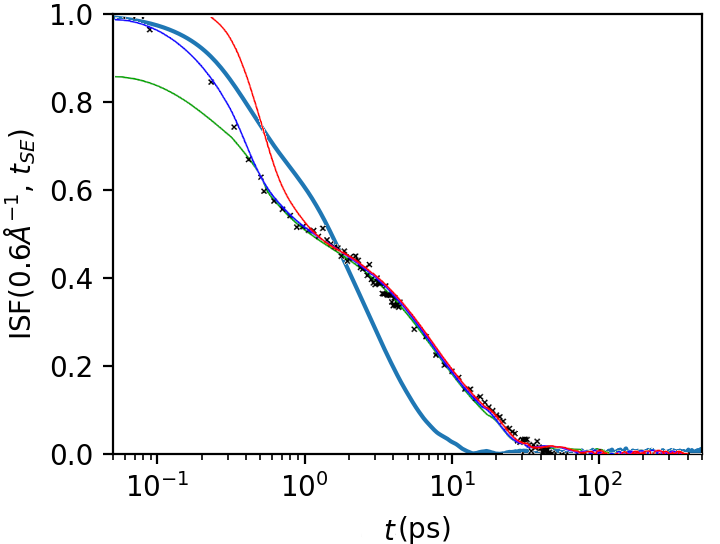
\includegraphics[width=1.0\textwidth]{md_isf_0.6_overlayed}
		\caption{The ISF of the adatom in the $\left[11\bar{2}\right]$ direction with $\left|\Delta{\vec{K}}\right|=\SI{0.6}{\per\angstrom}$. Overlayed in black crosses is HSEM data taken from \cite{Ward} for Lithium on Copper 111 at $\SI{140}{\kelvin}^{\text{\ref{rgb_lines}}}$.}
		\label{fig:md_isf_0.6}
	\end{subfigure}
	\hfill
	\begin{subfigure}{0.49\textwidth}
		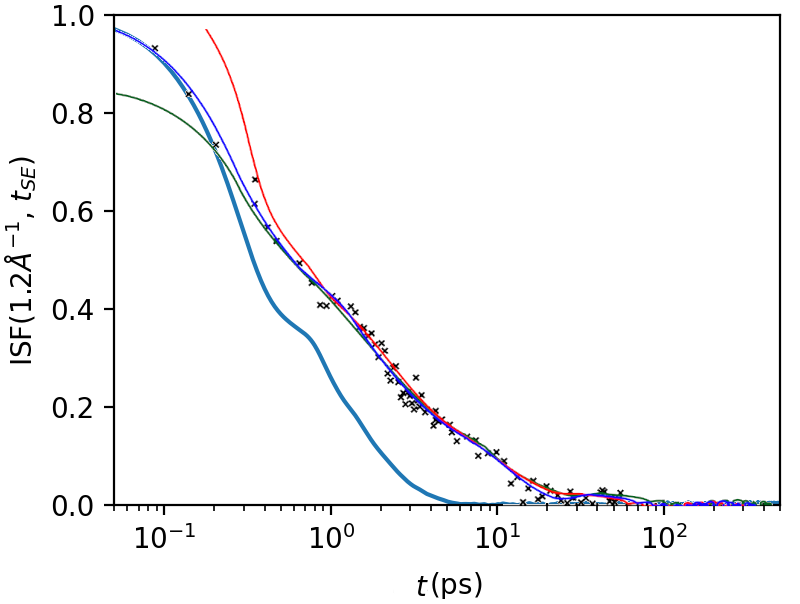
\includegraphics[width=1.0\textwidth]{md_isf_1.2_overlayed}
		\caption{The ISF of the adatom in the $\left[11\bar{2}\right]$ direction with $\left|\Delta{\vec{K}}\right|=\SI{0.6}{\per\angstrom}$. Overlayed in black crosses is HSEM data taken from \cite{Ward} for Lithium on Copper 111 at $\SI{140}{\kelvin}^{\text{\ref{rgb_lines}}}$.}
		\label{fig:md_isf_1.2}
	\end{subfigure}

	\begin{subfigure}{0.49\textwidth}
		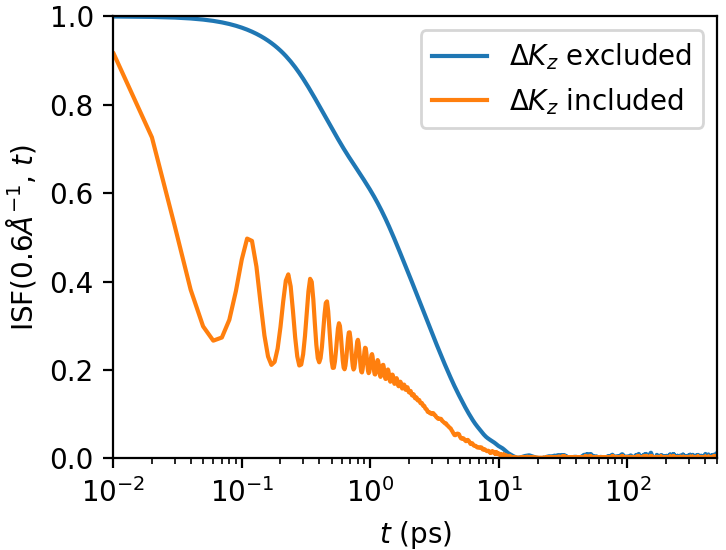
\includegraphics[width=1.0\textwidth]{isf_0.6_dkz_included}
		\caption{Two simulated ISFs with a parallel momentum transfer of $\SI{0.6}{\per\angstrom}$ in the $\left[11\bar{2}\right]$ direction. The momentum transfer used to calculate the orange ISF included an additional z-component of $\SI{9.93}{\per\angstrom}$ consistent with the assumptions of quasi-elastic scattering at the beam energy used in the Cambridge HSEM device \cite{HSEM}.}
		\label{fig:isf_0.6_dkz_included}
	\end{subfigure}
	\hfill
	\begin{subfigure}{0.49\textwidth}
		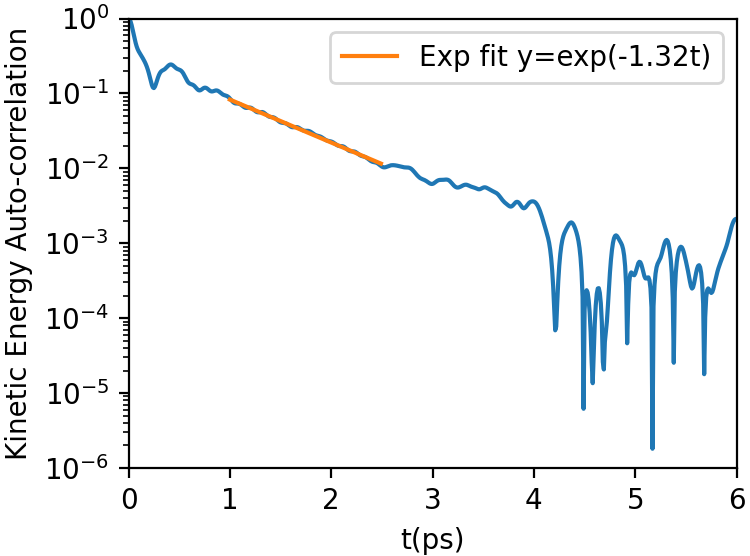
\includegraphics[width=1.0\textwidth]{md_kinetic_energy_autocorrelation}
		\caption{The kinetic energy auto-correlation function of the adatom on a log y-scale. The exponential fit suggests a naive estimate of the friction constant of around $\SI{1.32}{\per\pico\second}$ as per the discussion in Chapter \ref{sec:gle_interpretation}.}
		\label{fig:md_kinetic_energy_autocorrelation}
	\end{subfigure}
	
	\caption{Results of a $\SI{100}{\nano\second}$ run of the 3D molecular dynamics simulation constructed in Section \ref{sec:md_setup} at $\SI{140}{\kelvin}$ with Morse parameters summarized in Table \ref{table:fit_parameters}.}
	\label{fig:md_results}
\end{figure}


\begin{figure}
	\begin{subfigure}{0.49\textwidth}
		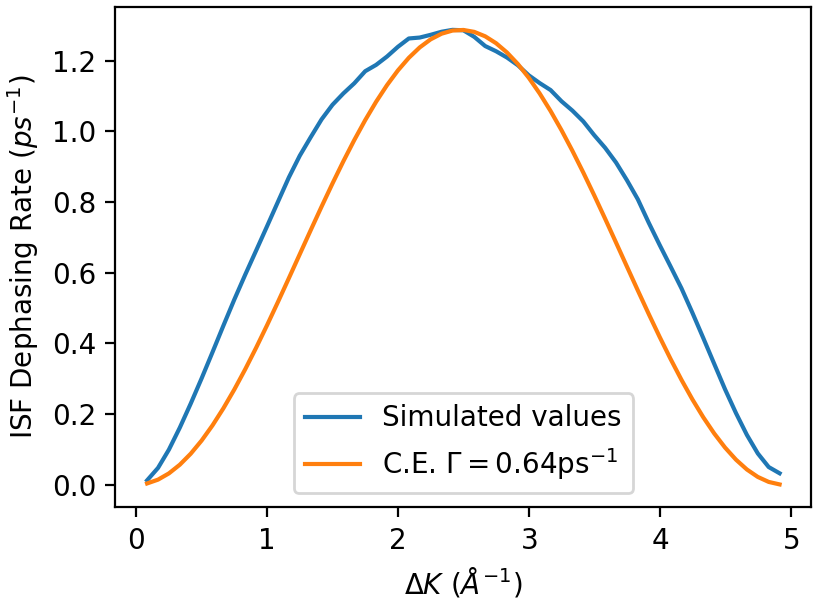
\includegraphics[width=1.0\textwidth]{alpha_deltak}
		\caption{The dephasing rate of the ISF as a function of $\left|\Delta{\vec{K}}\right|$ in the $\left[1\bar{1}0\right]$ direction alongside the theoretical form predicted by the Chudley-Elliot idealized hopping model \cite{Chudley_1961} at a rate of $\SI{0.64}{\per\pico\second}$.}
		\label{fig:alpha_deltak}
	\end{subfigure}
	\hfill	
	\begin{subfigure}{0.49\textwidth}
		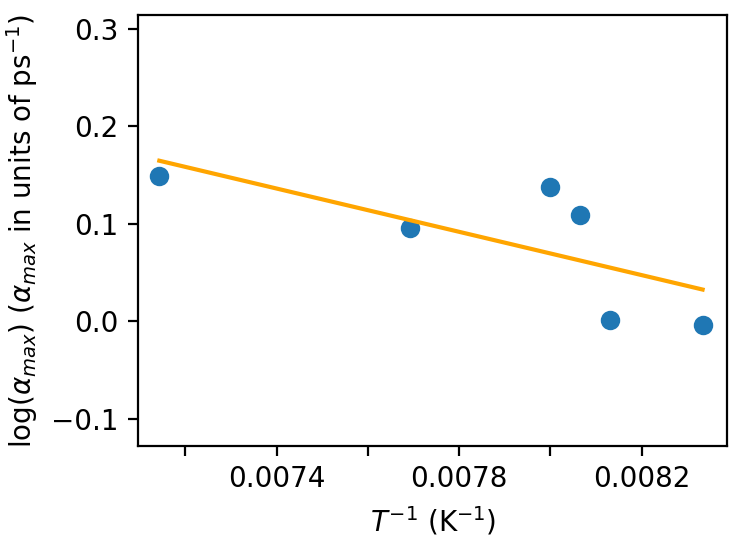
\includegraphics[width=1.0\textwidth]{ahrrenius_plot}
		\caption{Logarithm of the maximum ISF dephasing rate (proportional to the hopping rate) as a function of inverse temperature between $\SI{120}{\kelvin}$ and $\SI{140}{\kelvin}$. The linear fit suggests that the hopping process follows an Arrhenius law with activation energy $9.6\pm \SI{1.5}{\mev}$. The pre-exponential factor (y-cut on this plot) differs from the experimentally determined value.}
		\label{fig:ahrrenius_plot}
	\end{subfigure}

	\caption{Analysis of the hopping rate and activation energy of the molecular dynamics simulation.}	
\end{figure}

\chapter{Results of the GLE Simulations and Comparison with MD Simulations}

This chapter reports the results of GLE simulations performed on the parameter scales implied by the 3D MD simulations described in the previous chapter. The $\SI{7.4}{\tera\hertz}$ copper phonon cutoff frequency (Figure \ref{fig:phonon_dispersion_plot}) and energy auto-correlation decay rate of $\SI{1.32}{\per\pico\second}$ (Figure \ref{fig:md_kinetic_energy_autocorrelation}) inspired the investigation of $\tau$ on the order of $\frac{1}{f_{\text{cutoff}}} \sim \SI{e-1}{\pico\second}$ and $\eta \sim \SI{1}{\per\pico\second}$.

\section{Numerical Integrators and the Thermalisation of the GLE in a Background Potential} \label{sec:thermalization}

The use of velocity Verlet integration and the assumptions of the GLE in the presence of a background potential were evaluated using four background potentials:
\begin{itemize}
  \item No potential background
  \item A harmonic well
  \item A quartic well
  \item The corrugated potential extracted in Section \ref{sec:extract_potential}.
\end{itemize}
Each potential was simulated using three different integrator and memory kernel setups:
\begin{itemize}
	\item A velocity Verlet integrator with $\tau=\SI{0}{\ps}$
	\item A `modified' velocity Verlet integrator proposed in \cite{gronbech2013simple} with $\tau=\SI{0}{\ps}$
	\item A velocity Verlet integrator with $\tau=\SI{0.1}{\ps}$.
\end{itemize}
Each simulation was configured to run at $\SI{140}{\kelvin}$ assuming the fluctuation dissipation relation \ref{eq:tdomain_corr} holds. Each configuration was run $1000$ times for $\SI{500}{\pico\second}$ and the mean temperature of each run was recorded using $T=\frac{1}{k_B}\left<E_k\right>$. The results of these simulations are presented in Figure \ref{fig:thermalization_results}. The results demonstrate that the simulations with $\tau > 0$ exhibit more variance in general and all configurations had issues thermalizing with the corrugated potential. This suggests that either the fluctuation dissipation relation \ref{eq:tdomain_corr} does not hold for general background potentials or that the interplay between Velocity Verlet integrators and the GLE in a highly non-linear background force cause the simulation to exhibit a slightly incorrect temperature. In the GLE simulations which follow, small temperature adjustments were made to counteract this effect when appropriate. 

\begin{figure}
	\makebox[\textwidth][c]{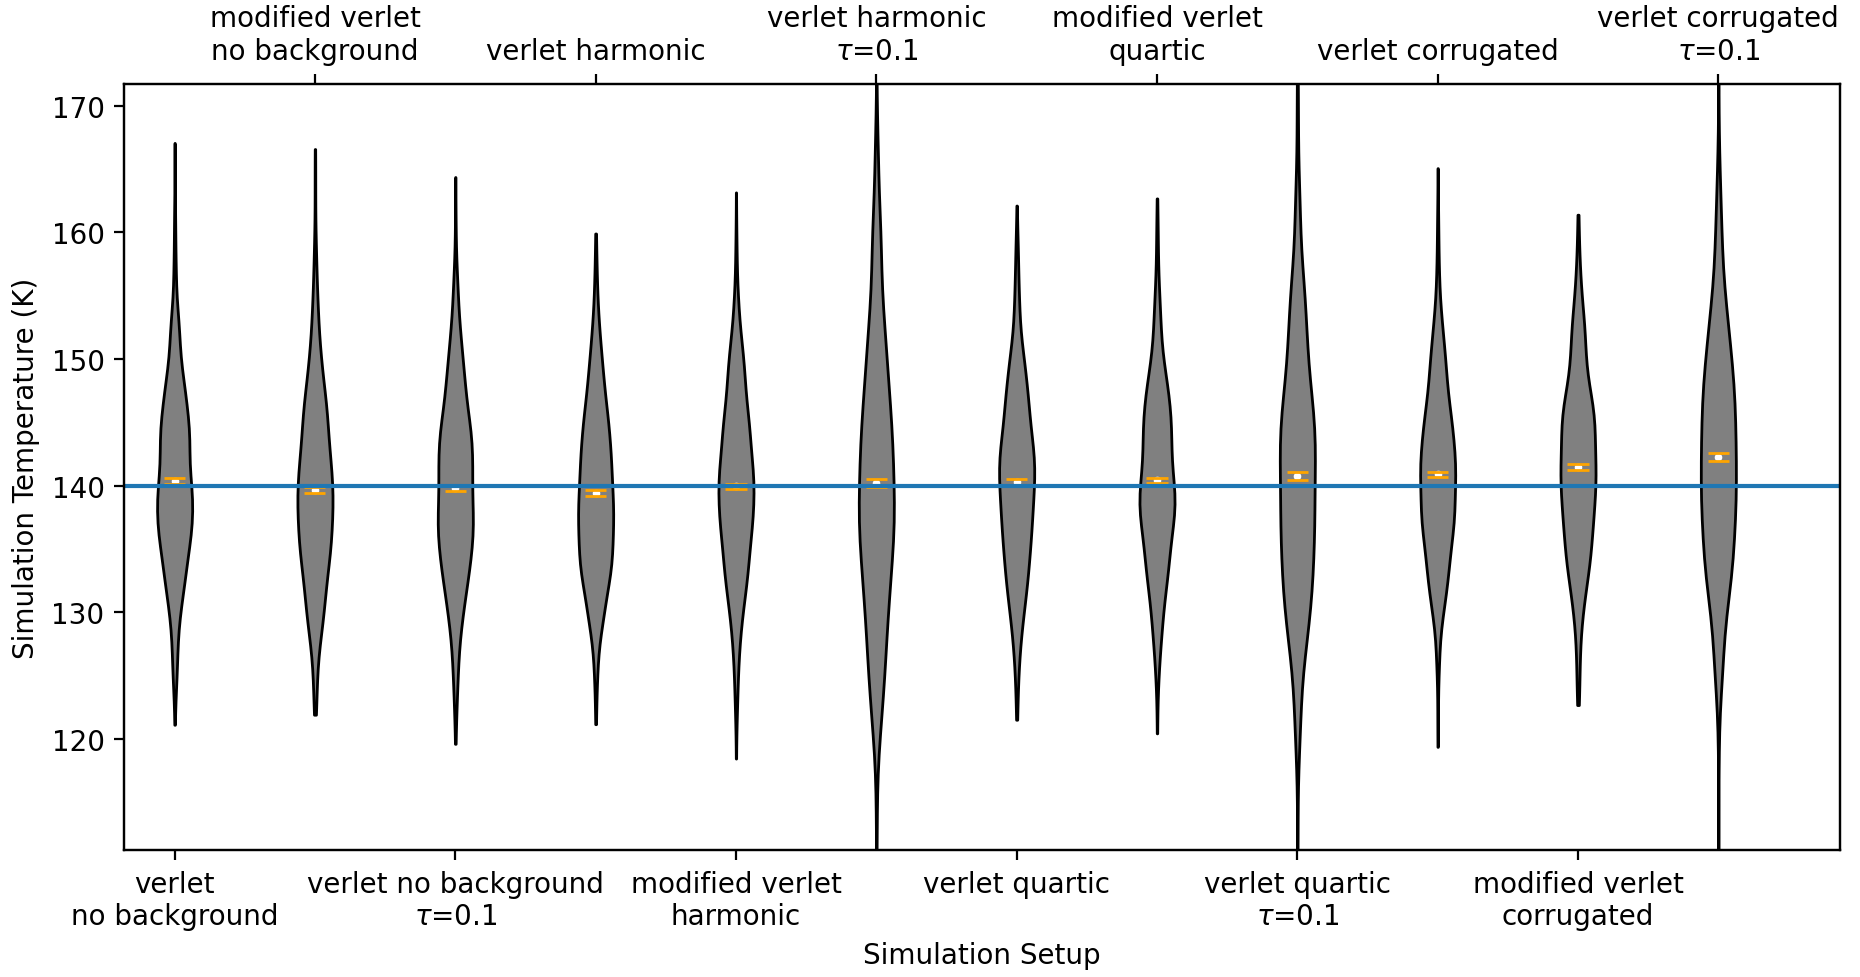
\includegraphics[width=1.2\textwidth]{gle_thermalization}}
	\caption{Distributions of the simulated temperature of various GLE simulation setups. Each configuration was run $1000$ times using the fluctuation-dissipation relation \ref{eq:tdomain_corr} at $\SI{140}{\kelvin}$ for $\SI{500}{\pico\second}$. Kernel density plots are vertically oriented showing the distribution of a single simulation temperature sample. White points indicate the mean value of a configuration and the small orange lines indicate a $\mu \pm 1\bar{\sigma}$ interval of the sample mean standard deviation $\bar{\sigma}=\frac{\sigma}{\sqrt{1000}}$.}
	\label{fig:thermalization_results}
\end{figure}

\section{Effects of the GLE Parameters on Simulated ISFs}

\begin{figure}
	\begin{subfigure}{1.0\textwidth}
		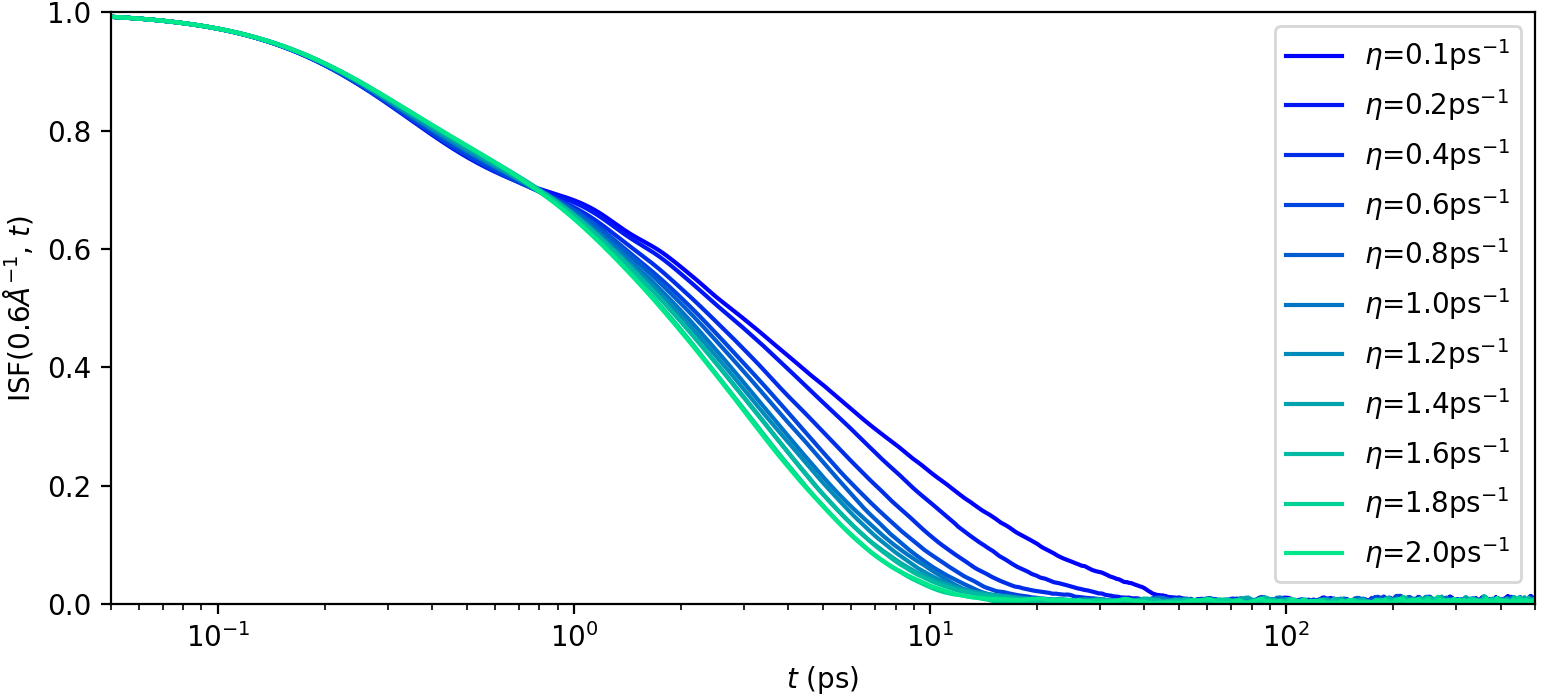
\includegraphics[width=1.0\textwidth]{vary_eta_0.6}
		\caption{ISFs on a log x-scale across a range of $\eta$ values for fixed $\tau=\SI{0.1}{\ps}$.}
		\label{fig:vary_eta_0.6}
	\end{subfigure}	
	\begin{subfigure}{0.49\textwidth}
		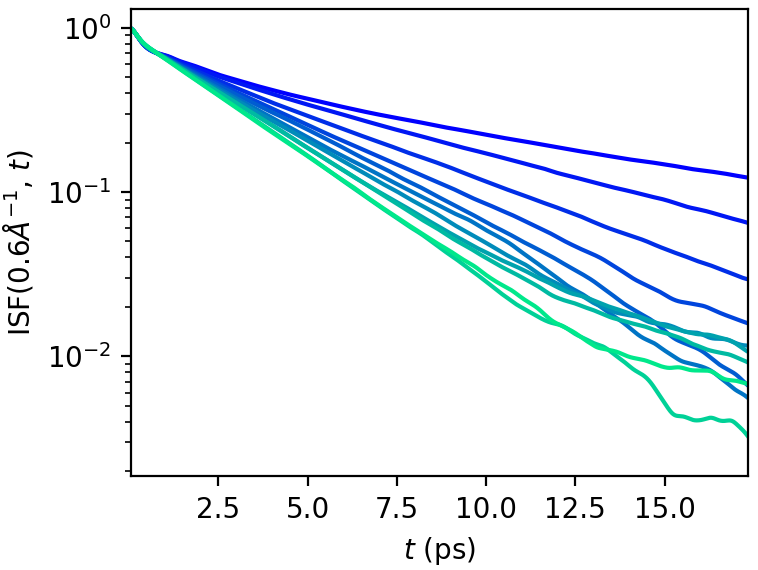
\includegraphics[width=1.0\textwidth]{vary_eta_0.6_log}
		\caption{ISFs on a log y-scale across a range of $\eta$ values for fixed $\tau=\SI{0.1}{\ps}$. The gradient of the straight line segments give the ISF dephasing rate. Shares a legend with Figure \ref{fig:vary_eta_0.6}.}
		\label{fig:vary_eta_0.6_log}
	\end{subfigure}
	\hfill
	\begin{subfigure}{0.49\textwidth}
		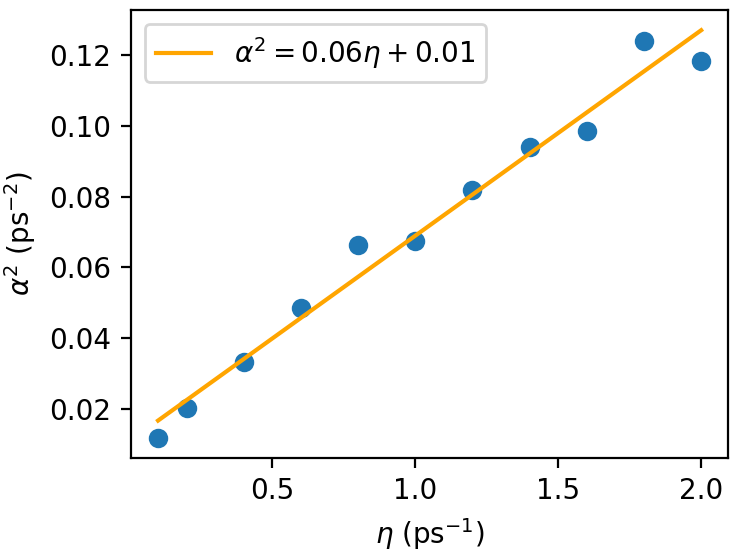
\includegraphics[width=1.0\textwidth]{alpha_vs_eta}
		\caption{The square of the dephasing rate of the ISFs in Figure \ref{fig:vary_eta_0.6} as a function of $\eta$. The form suggests a dependence of the form $\alpha \propto \sqrt{\eta}$.}
		\label{fig:alpha_vs_eta}
	\end{subfigure}
	\caption{ISFs in the $\left[1\bar{1}0\right]$ direction produced by GLE simulations using the corrugated potential obtained in Section \ref{sec:extract_potential} across a range of $\eta$ values with fixed $\tau=\SI{0.1}{\ps}$. All runs were performed at $140K$ for $\SI{100}{\ns}$ with a $\SI{1}{\fs}$ time-step.}
	\label{fig:vary_eta_all}
\end{figure}


\begin{figure}
	\begin{subfigure}{1.0\textwidth}
		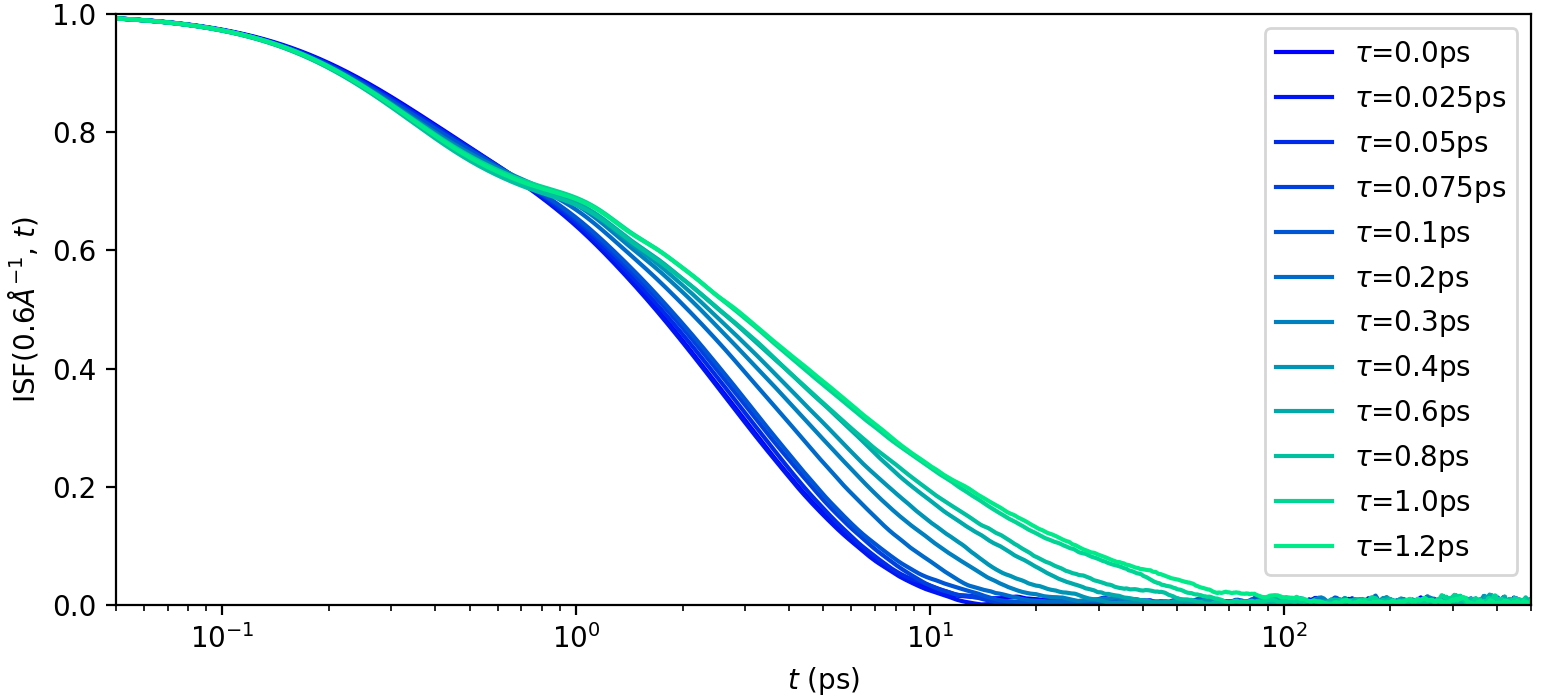
\includegraphics[width=1.0\textwidth]{vary_tau_0.6}
		\caption{ISFs on a log x-scale across a range of $\tau$ values for fixed $\eta=\SI{1.32}{\ips}$.}
		\label{fig:vary_tau_0.6}
	\end{subfigure}

	\begin{subfigure}{0.49\textwidth}
		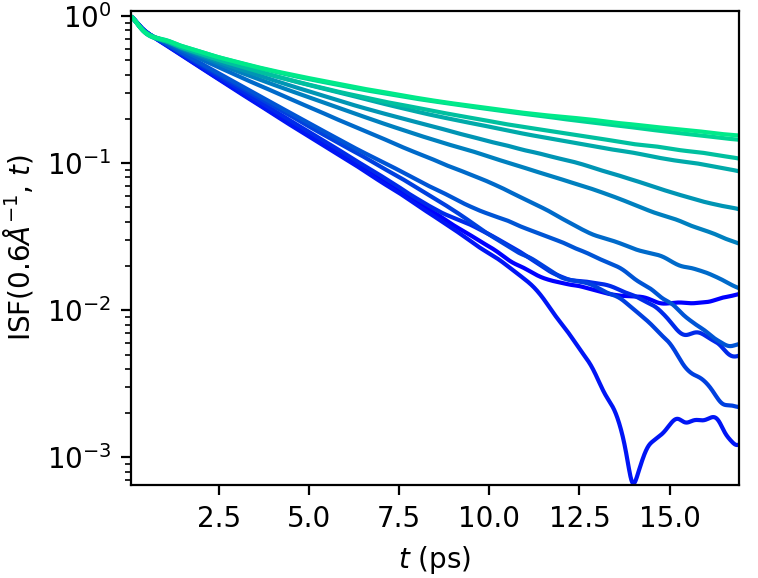
\includegraphics[width=1.0\textwidth]{vary_tau_0.6_log}
		\caption{ISFs on a log y-scale across a range of $\tau$ values for fixed $\eta=\SI{1.32}{\ips}$. The gradient of the straight line segments give the ISF dephasing rate. Shares a legend with Figure \ref{fig:vary_tau_0.6}.}
		\label{fig:vary_tau_0.6_log}
	\end{subfigure}
	\hfill	
	\begin{subfigure}{0.49\textwidth}
		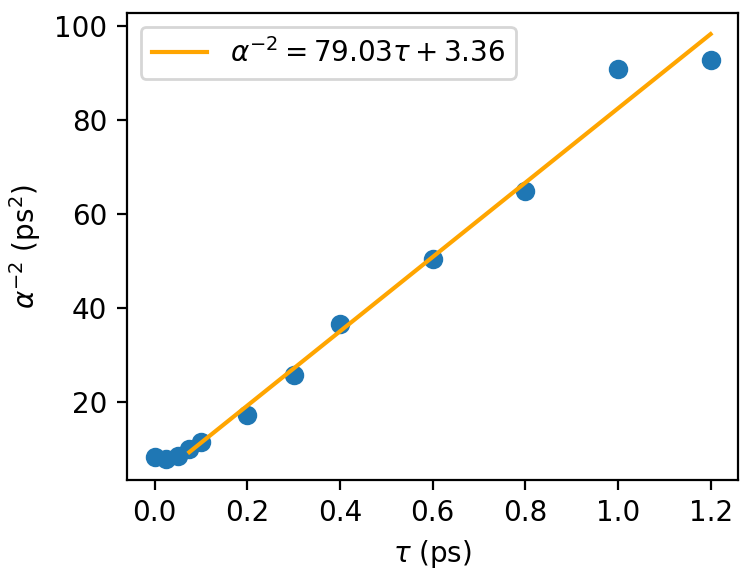
\includegraphics[width=1.0\textwidth]{alpha_vs_tau}
		\caption{The reciprocal of the dephasing rate of the ISFs in Figure \ref{fig:vary_tau_0.6} as a function of $\tau$.}
		\label{fig:alpha_vs_tau}
	\end{subfigure}
	\caption{ISFs in the $\left[1\bar{1}0\right]$ direction produced by GLE simulations using the corrugated potential obtained in Section \ref{sec:extract_potential} across a range of $\tau$ values with fixed $\eta=\SI{1.32}{\ips}$. All runs were performed at $140K$ for $\SI{100}{\ns}$ with a $\SI{1}{\fs}$ time-step.}
	\label{fig:vary_tau_all}
\end{figure}

Figures \ref{fig:vary_eta_all} \& \ref{fig:vary_tau_all} show the outcome of a number of $\SI{100}{\ns}$ GLE runs at $\SI{140}{\kelvin}$ over a range of values of $\eta$ and $\tau$.  

All runs show long term behavior of hopping between neighboring sites at a rate which varies with the value of $\tau$ and $\eta$. The effect of varying $\tau$ around $\tau=\SI{0}{\ps}$ is small as on this scale $\tau$ only affects very high frequency noise components $>\SI{10}{\thz}$ which average out on the timescale of hopping anyway. As $\tau$ increases past $\SI{e-1}{\ps}$, the simulations exhibit a slower hopping rate since $\tau$ begins to strongly suppress the frequency range which drive hopping on the timescale of $\SI{1}{\ps}$.

The hopping rate is observed to increase with the friction parameter $\eta$. This is an expected result within transition state theory \cite{BLIGAARD2008255} as $\eta$ quantifies the coupling between the noise of the system and the particle. $\eta$ thereby determines the rate at which the particle changes its energy. With no friction, the particle's total energy can never change and must therefore stay bound to its local absorption site. 

The results in Figure \ref{fig:alpha_vs_eta} \& \ref{fig:alpha_vs_tau} suggest an asymptotic relationship of the form $\alpha \propto \sqrt{\frac{\eta}{\tau}}$. While this origin of this relationship is not well understood, it is interesting to notice that within transition state theory, the pre-exponential factor of a reaction is inversely proportional to the effective mass of the system in its transition state \cite{BLIGAARD2008255}. Furthermore the GLE is introduced to model systems in which the particles driving the stochastic force are no longer of negligible mass \cite{Kubo}. It is proposed that this non-negligible mass scale affects the system's transition state effective mass linearly in $\tau$ in this parameter regime, however, this assumption is yet to be justified.   

The parameters show no effect on the ISFs at very short timescales since the thermal velocity of lithium is independent of $\eta$ and $\tau$.

\section{Comparison of ISFs Produced Using the GLE and the MD Simulation}

\begin{figure}
	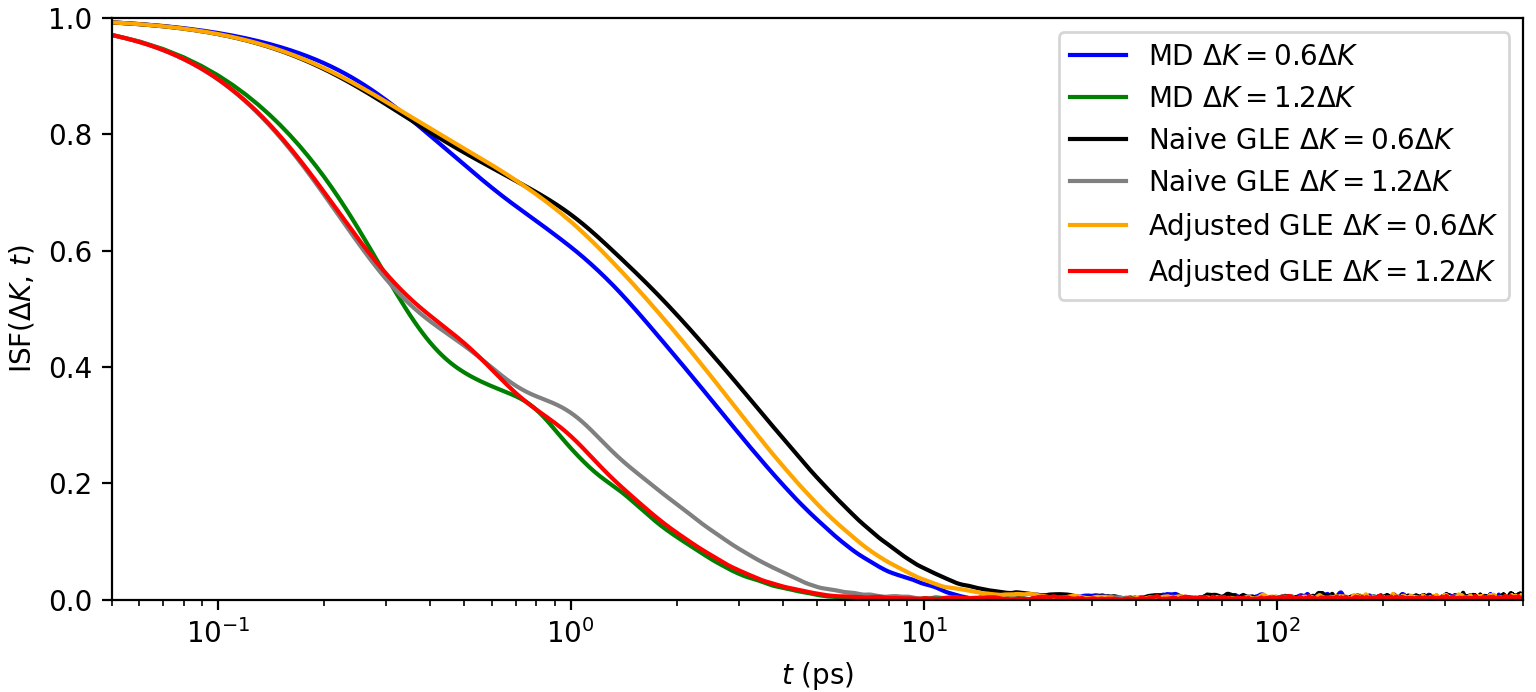
\includegraphics[width=1.0\textwidth]{md_vs_gle}
	\caption{Comparison of ISFs produced using: 1. the 3D MD simulation, 2. the GLE simulation with the naive parameter estimates $\tau=\frac{1}{f_c}=\SI{0.135}{\ps}$ and $\eta=\SI{1.32}{\ips}$ (see Figure \ref{fig:md_kinetic_energy_autocorrelation}), and 3. The GLE with parameters adjusted to $\tau=\SI{0.1}{\ps}$ and $\eta=\SI{1.9}{\ips}$ using the relationships implied by Figures \ref{fig:vary_eta_all} \& \ref{fig:vary_tau_all} to fit the MD dephasing rate.}
	\label{fig:md_vs_gle}
\end{figure}

Following the discussions in Chapter \ref{sec:gle_interpretation},  the phonon cutoff frequency, $f_c=\SI{7.4}{\thz}$, determined in Section \ref{sec:phonon_spectrum} along with the MD kinetic energy auto-correlation decay rate shown in Figure \ref{fig:md_kinetic_energy_autocorrelation} provide a `naive' estimate for reasonable GLE parameters with which to compare the GLE to the MD simulation. Figure \ref{fig:md_vs_gle} compares ISFs produced using the MD simulation to those produced with the GLE. This figure includes an additional ISF produced using the GLE parameters adjusted using the relationships in Figures \ref{fig:vary_eta_all} \& \ref{fig:vary_tau_all} to match the MD simulation's dephasing rate.

These results show that the GLE does a very good job of reproducing the ISF of the original MD simulation even when using the naive estimates presented. In particular, the dephasing rate can be exactly matched through simple adjustments of $\eta$ and $\tau$. The remaining discrepancies between the ISFs are attributed to the precise shape of the potential energy surface used in the GLE (including any errors produced in the extraction process) and differences between the noise spectrum seen in the simulation and the spectrum of the exponential memory kernel. 


\chapter{Conclusions and Outlook}

A careful analysis of the thermalization properties of the GLE in various background potentials has been performed. The results show that the introduction of a cutoff in the noise spectrum introduces additional variance in the temperature fluctuations of the system. Additionally, the Velocity Verlet integration technique is shown to produce a mean simulation temperature which is $1-2\%$ too high when applied to the GLE in a corrugated potential.

A first-principles derivation of the ISF and energy auto-correlation function of a particle obeying the GLE in a harmonic background potential has been presented. These expressions have been evaluated analytically for the first time in the special case of an exponential memory kernel, $K(t)=\frac{1}{\tau}e^{-\frac{t}{\tau}}$, and used to provide interpretations of the GLE parameters in the small $\tau$ regime. These results serve as a useful tool for extracting GLE parameters from the ISF and energy auto-correlation function of a MD simulation. These parameter extraction techniques have potential to be applied directly to experimental data.

A semi-realistic, classical, 3D molecular dynamics simulation of lithium on copper(111) has been constructed with one to two orders of magnitude more substrate atoms than similar simulations in previous work. The simulation has been fully validated, analyzed and compared with the known properties of lithium on copper(111). In particular, the simulation faithfully reproduces the phonon spectrum of real copper (with a phonon cutoff frequency of $\SI{7.4}{\tera\hertz}$) and therefore fully captures the classical notion of the stochastic noise seen by an adatom. The simulation has been used to show that this classical simulation of lithium on copper(111) fails to reproduce the pre-exponential factor of the hopping rate as well as ratio of fast to slow motion seen in the experimental data.

A corresponding 2D GLE simulation with an exponential memory kernel has been constructed with parameters extracted directly from the MD simulation using the aforementioned parameter extraction technique. This simulation has been shown to produce ISFs which match the MD simulations extremely well. Together with results from \cite{Ward} which show that the experimental lithium on copper data is explained using a GLE with a frequency cutoff of around $\SI{1.25}{\tera\hertz}$, this leads to the conclusion that the effective noise seen by lithium on copper(111) is far more band limited than a classical model would predict. This suggests an additional noise filter of unknown origin is present in the system which effectively band limits the noise spectrum seen by the lithium to around $\SI{1.25}{\tera\hertz}$. Since lithium is a very light atom with a thermal de Broglie wavelength on the order of $\SI{0.5}{\angstrom}$ (smaller than but still comparable to the copper lattice spacing of $\SI{2.54}{\angstrom}$), this filter may be quantum mechanical in nature.

Using a corrugated potential extracted from the full MD simulation, the effect of the parameters $\eta$ and $\tau$ on the ISFs produced in GLE simulations are derived numerically. The simulation results re-affirm the expectation that a frequency cutoff much higher than the typical hopping rate observed in the MD simulation of around $\SI{0.93}{\ips}$(corresponding to very small $\tau$) has very little effect on the long term hopping rate of the particle. The numerical results suggest an asymptotic relationship of $\alpha \propto \sqrt{\frac{\eta}{\tau}}$ for the ISF dephasing rate at larger $\tau$ which is not fully understood and may provide an avenue for further research within transition state theory. 

\appendix

\chapter{Derivation of Analytic Expressions for the GLE in a Harmonic Well} \label{apx:analytic_gle_appendix}

This appendix provides a first-principles derivation of analytic expressions for the ISF and energy auto-correlation function of the GLE within a background harmonic potential well. Some of these expressions have been independently derived in an alternative form in \cite{Townsend_2018}, however some of these expressions are evaluated for the first time. 

\section{The Greens Function of the GLE in a Harmonic Potential}

The generalized Langevin equation is given by

$$
m\ddot{x} + m\eta \int_{-\infty}^{\infty} dt' K(t - t')v(t') + m\omega_0^2 x = \int_{-\infty}^{\infty} dt' K(t - t')f(t')
$$
\\
for an arbitrary memory kernel $K(t)$ in a harmonic potential background with natural frequency $\omega_0$. The random force is given by $f(t)$ and has variance $\left<f_i(t)f_j(t')\right>=\delta_{ij}\delta(t-t')\sigma^2 = \delta_{ij}\delta(t-t')2kTm\eta$ where $m$ is the particle mass and $\eta$ is a friction constant in units of inverse time. If required, causality is assumed to be implicit to $K(t)$. Fourier transforming both sides and using the convolution theorem,

$$
-m\omega^2 \tilde{x}(\omega) + i m \eta \omega \tilde{x}(\omega) \tilde{K}(\omega) + m\omega_0^2 \tilde{x}(\omega) = \tilde{f}(\omega) \tilde{K}(\omega)
$$
$$
\implies \tilde{x} = \frac{1}{m} \frac{\tilde{f} \tilde{K}}{-\omega^2 + i \eta \omega \tilde{K} + \omega_0^2} = \frac{1}{m} \tilde{f} \tilde{F}.
$$
\\
The Green's function of the GLE, $F(t)$, has been introduced so that the trajectory of a particle is given by $x(t) = \frac{1}{m}\int_{-\infty}^{\infty}dt'F(t-t')f(t')$.

\section{The ISF of a Particle Obeying the GLE in a Harmonic Potential Well \label{isf_gle_well}}
\label{ch:gle_derivation}

The intermediate scattering function is given by the spatial Fourier transform of the van Hove pair correlation function $G\left(\vec{r},t\right)$. For a single particle, this is equivalent to $P\left(\vec{r}, t\right)$, the probability of finding the particle at $\vec{r}$ at time $t$ given that it was at the origin at $t=0$ \cite{vanhove}. For a single particle trajectory, $\vec{r}(t)$, this given by 

$$
ISF(\Delta \vec{K}, t) = \int d\vec{R} e^{-i \Delta \vec{K} \cdot \left(\vec{R} - \vec{r}(0)\right)} P(\vec{R}, t) = \int d\vec{R} e^{-i \Delta \vec{K} \cdot \left(\vec{R} - \vec{r}(0)\right)} \delta(\vec{R} - \vec{r}(t)) = e^{-i \Delta \vec{K} \cdot \left(\vec{r}(t) - \vec{r}(0)\right)}
$$
\\
Using the Green's function $F(t)$, $\vec{r}(t) - \vec{r}(0) = \frac{1}{m} \int \frac{d\omega}{2\pi} \left(e^{i\omega t} - 1\right) \tilde{F} \tilde{f}$. Substituting this into the above results in

$$
ISF(\Delta \vec{K}, t) = e^{- \frac{i}{m} \int \frac{d\omega}{2\pi} \left(e^{i\omega t} - 1\right) \tilde{F} \left(\Delta \vec{K} \cdot \tilde{f}\right))}
$$
\\
Expanding out the exponential and taking an ensemble average yields
$$
\left<ISF(\Delta \vec{K}, t)\right> = \sum_{n=0}^{\infty} \left(- \frac{i}{m}\right)^n \frac{1}{n!} \left< \left( \int \frac{d\omega}{2\pi} \left(e^{i\omega t} - 1\right) \tilde{F} \left(\Delta \vec{K} \cdot \tilde{f}\right)\right)^n\right>
$$
\\
\begin{equation}
= \sum_{n=0}^{\infty} \left(- \frac{i}{m}\right)^n \frac{1}{n!} \left( \int \frac{d\omega}{2\pi} \left(e^{i\omega t} - 1\right) \tilde{F}\right)^n \left< \left(\Delta \vec{K} \cdot \tilde{f}\right)^n\right> \label{eq:isf_1}
\end{equation}
\\
I have abused notation in the last line to summarize $n$ integrals over $\omega_1$ through $\omega_n$. For the remainder of the derivation it is assumed that the random force is both isotropic and has a zero mean. These constraints can be relaxed and this may be used to model materials with an-isotropic noise spectra such as materials with large differences in the phonon frequency cut-offs for the various phonon polarization directions.
Taking a closer look at $\left< \left(\Delta \vec{K} \cdot \tilde{f}\right)^n\right>$ in one dimension,
$$
\left< \left(\Delta \vec{K} \cdot \tilde{f}\right)^n\right> = \left|\Delta \vec{K}\right|^n \left< \tilde{f}\left(\omega_1\right) \ldots \tilde{f}\left(\omega_n\right)\right>.
$$
From the isotropy and zero mean of $f$ it follows that the above vanishes for odd $n$. For even $n$, the expectation is given by summing over the product of all possible pairwise expectations of $\left< \tilde{f}\left(\omega_1\right) \ldots \tilde{f}\left(\omega_n\right) \right>$ \footnote{This follows from the vanishing higher order cumulants of white noise. See David Tong's notes \cite{Tong}.},
$$
\left< \left(\Delta \vec{K} \cdot \tilde{f}\right)^{2n}\right> = \left|\Delta \vec{K}\right|^{2n} \frac{1}{2^nn!} \sum_P \left< \tilde{f}\left(\omega_{P_1}\right) \tilde{f}\left(\omega_{P_2}\right)\right> \ldots \left< \tilde{f}\left(\omega_{P_{2n-1}}\right) \tilde{f}\left(\omega_{P_{2n}}\right)\right>
$$
$$
= \left|\Delta \vec{K}\right|^{2n} \frac{\left(2\pi\sigma^2\right)^n}{2^nn!} \sum_P \delta\left(\omega_{P_1} + \omega_{P_2}\right) \ldots \delta\left(\omega_{P_{2n-1}} + \omega_{P_{2n}}\right)
$$
The last step follows immediately from the Fourier transform of $\left<f(t)f(t')\right>=\delta(t-t')\sigma^2$. Substituting into \ref{eq:isf_1} yields
$$
\sum_{n=0}^{\infty} \left(- \frac{i}{m}\right)^{2n} \frac{1}{(2n)!} \left( \int \frac{d\omega}{2\pi} \left(e^{i\omega t} - 1\right) \tilde{F}\right)^{2n} \left|\Delta \vec{K}\right|^{2n} \frac{\left(2\pi\sigma^2\right)^n}{2^nn!} \sum_P \delta\left(\omega_{P_1} + \omega_{P_2}\right) \ldots \delta\left(\omega_{P_{2n-1}} + \omega_{P_{2n}}\right)
$$
$$
= \sum_{n=0}^{\infty} \left(- \frac{i}{m}\right)^{2n} \frac{1}{(2n)!} \left( \int \frac{d\omega}{2\pi} \left|\left(e^{i\omega t} - 1\right) \tilde{F}\right|^2\right)^{n} \left|\Delta \vec{K}\right|^{2n} \frac{\left(\sigma^2\right)^n(2n)!}{2^nn!}
$$
$$
= \sum_{n=0}^{\infty} \frac{1}{n!} \left(-\frac{|\Delta \vec{K}|^2 \sigma^2}{m^2} \int \frac{d\omega}{2\pi}\left(1 - \cos\left(\omega t\right)\right) \left| \tilde{F} \right|^2\right)^n
$$
\begin{equation}
= \exp\left(-\frac{|\Delta \vec{K}|^2 \sigma^2}{m^2} \int \frac{d\omega}{2\pi}\left(1 - \cos\left(\omega t\right)\right) \left| \tilde{F} \right|^2\right) \label{isf_explicity_norm}
\end{equation}
\\
From equation \ref{isf_explicity_norm} it is clear the ISF is normalized to 1 at $t=0$. Since $F(t)$ is a real function, $|\tilde{F}|^2$ must be even, so $\int \frac{d\omega}{2\pi}\left(\cos\left(\omega t\right)\right) \left| \tilde{F} \right|^2 = \int \frac{d\omega}{2\pi}\ e^{i \omega t} \left| \tilde{F} \right|^2$ which is nothing but the auto-correlation of $F(t)$ (denoted by $C_F(t)$). Moreover, $\int \frac{d\omega}{2\pi}\left| \tilde{F} \right|^2$, by the residue theorem, is nothing more than the sum of the residues of the poles of $\left|\tilde{F}\right|^2$ in the upper (or lower since the function is symmetric) half complex plane. So our final expression for a general isotropic memory kernel is
\begin{equation}
\left<ISF(\Delta \vec{K}, t)\right> = ISF\left(\Delta \vec{K}, \infty \right)\exp\left(\frac{|\Delta \vec{K}|^2 \sigma^2}{m^2} C_F\left(t\right) \right). \label{isf_compact} 
\end{equation}
\\
We are able to define $ISF\left(\Delta \vec{K}, \infty \right)= \exp \left( -\frac{|\Delta \vec{K}|^2 \sigma^2}{m^2} \int \frac{d\omega}{2\pi} \left| \tilde{F} \right|^2 \right)$ since at large times, provided $F(t \rightarrow \infty)$ tends to $0$ fast enough, $C_F(t \rightarrow \infty) = 0$.

\section{The Kinetic Energy Auto-correlation Function \label{kinetic_autocorrelation}}

The velocity of a particle obeying the GLE may be written in terms of the Green's function as $\dot{x}(t) = \frac{i}{m}\int\frac{d\omega}{2\pi} \omega e^{i\omega t}\tilde{f}(\omega)\tilde{F}(\omega)$. The kinetic energy auto-correlation function at equilibrium is therefore given by
$$
\left<E(0)E(t)\right>=\frac{m^2}{4}\left<\dot{x}(0)^2\dot{x}(t)^2\right>=\frac{1}{4m^2}\left(\int\frac{d\omega}{2\pi}\omega\tilde{F}\right)^4 e^{i\left(\omega_3 + \omega_4 \right)t} \left<\left(\tilde{f}(\omega_1)\cdot\tilde{f}(\omega_2)\right)\left(\tilde{f}(\omega_3)\cdot\tilde{f}(\omega_4)\right)\right>
$$
Where I have once again abused notation to summarize four integrals over $\omega_1\cdots\omega_4$. By expanding the dot product component wise and taking care to sum over all the products of pairwise expectations (as in \cite{Tong}), in two dimensions,  $\left<\left(\tilde{f}(\omega_1)\cdot\tilde{f}(\omega_2)\right)\left(\tilde{f}(\omega_3)\cdot\tilde{f}(\omega_4)\right)\right>$ is given by 

$$
2\left(2\pi\sigma^2\right)^2\left(2\delta(\omega_1+\omega_2)\delta(\omega_3+\omega_4) + \delta(\omega_1+\omega_2)\delta(\omega_3+\omega_4) + \delta(\omega_1+\omega_2)\delta(\omega_3+\omega_4)\right).
$$
\\
Therefore in 2 dimensions,
$$
\left<E(0)E(t)\right>=\frac{\sigma^4}{m^2}\left(\left(\int\frac{dw}{2\pi}\omega^2\left|\tilde{F}(\omega)\right|^2\right)^2 + \left(\int\frac{dw}{2\pi}e^{i\omega t}\omega^2\left|\tilde{F}(\omega)\right|^2\right)^2\right).
$$

\section{Simplifications for an Exponential Memory Kernel}

\subsection{Evaluating integrals of the form $\int\frac{dw}{2\pi} g\left(\omega\right) \left|\tilde{F}\left(\omega\right)\right|^2$} 

Given an exponential memory kernel $K(t) = \theta(t) \frac{1}{\tau} e^{-\frac{t}{\tau}}$, integrals of the form $\int\frac{dw}{2\pi} g\left(\omega\right) \left|\tilde{F}\left(\omega\right)\right|^2$ for well behaved functions $g$ may be evaluated using the residue theorem. The Fourier transform of the kernel is given by $\tilde{K}\left(\omega\right) = \frac{1}{1+i\omega\tau}$ which may be easily verified using the residue theorem. Substituting $\tilde{K}$ into the formula for $\tilde{F}$ and simplifying gives
$$
\tilde{F} = \frac{-1}{i\tau\omega^3 + \omega^2 - i\omega(\omega_0^2\tau + \eta) - \omega_0^2} =: \frac{-1}{P(\omega)}
$$
Where the 3rd order polynomial $P(\omega)$ has been introduced. Since $P(i\omega)$ is a polynomial with real co-efficients, it follows from the complex conjugate root theorem that for any root $z$ of $P(\omega)$, $-z^*$ is also a root of $P(\omega)$. This allows us to make the ansatz that $P$ may be factorized as $P(\omega) = i\tau\left(\omega - \chi\right)\left(\omega + \chi^*\right)\left(\omega - i\eta_1\right)$ for some $\chi\in\mathbb{C}$ and ${\eta_1\in\mathbb{R}}$. While it is possible that in certain regions of the $\tau,\eta,\omega_0$ parameter space $P(\omega)$ has three imaginary roots (analogous to the damped harmonic oscillator or \cite{Townsend_2018}), these parameter ranges were not encountered in the course of this project and were not further investigated. Furthermore, if the Greens function $F(t)$ is to be causal, all three roots must occur in the upper half plane \cite{Runkel}. We therefore find that the pole structure of $\left|\tilde{F}\right|^2$, as shown in Figure \ref{fig:pole_structure}. 
\\
\begin{figure}
	\centering
	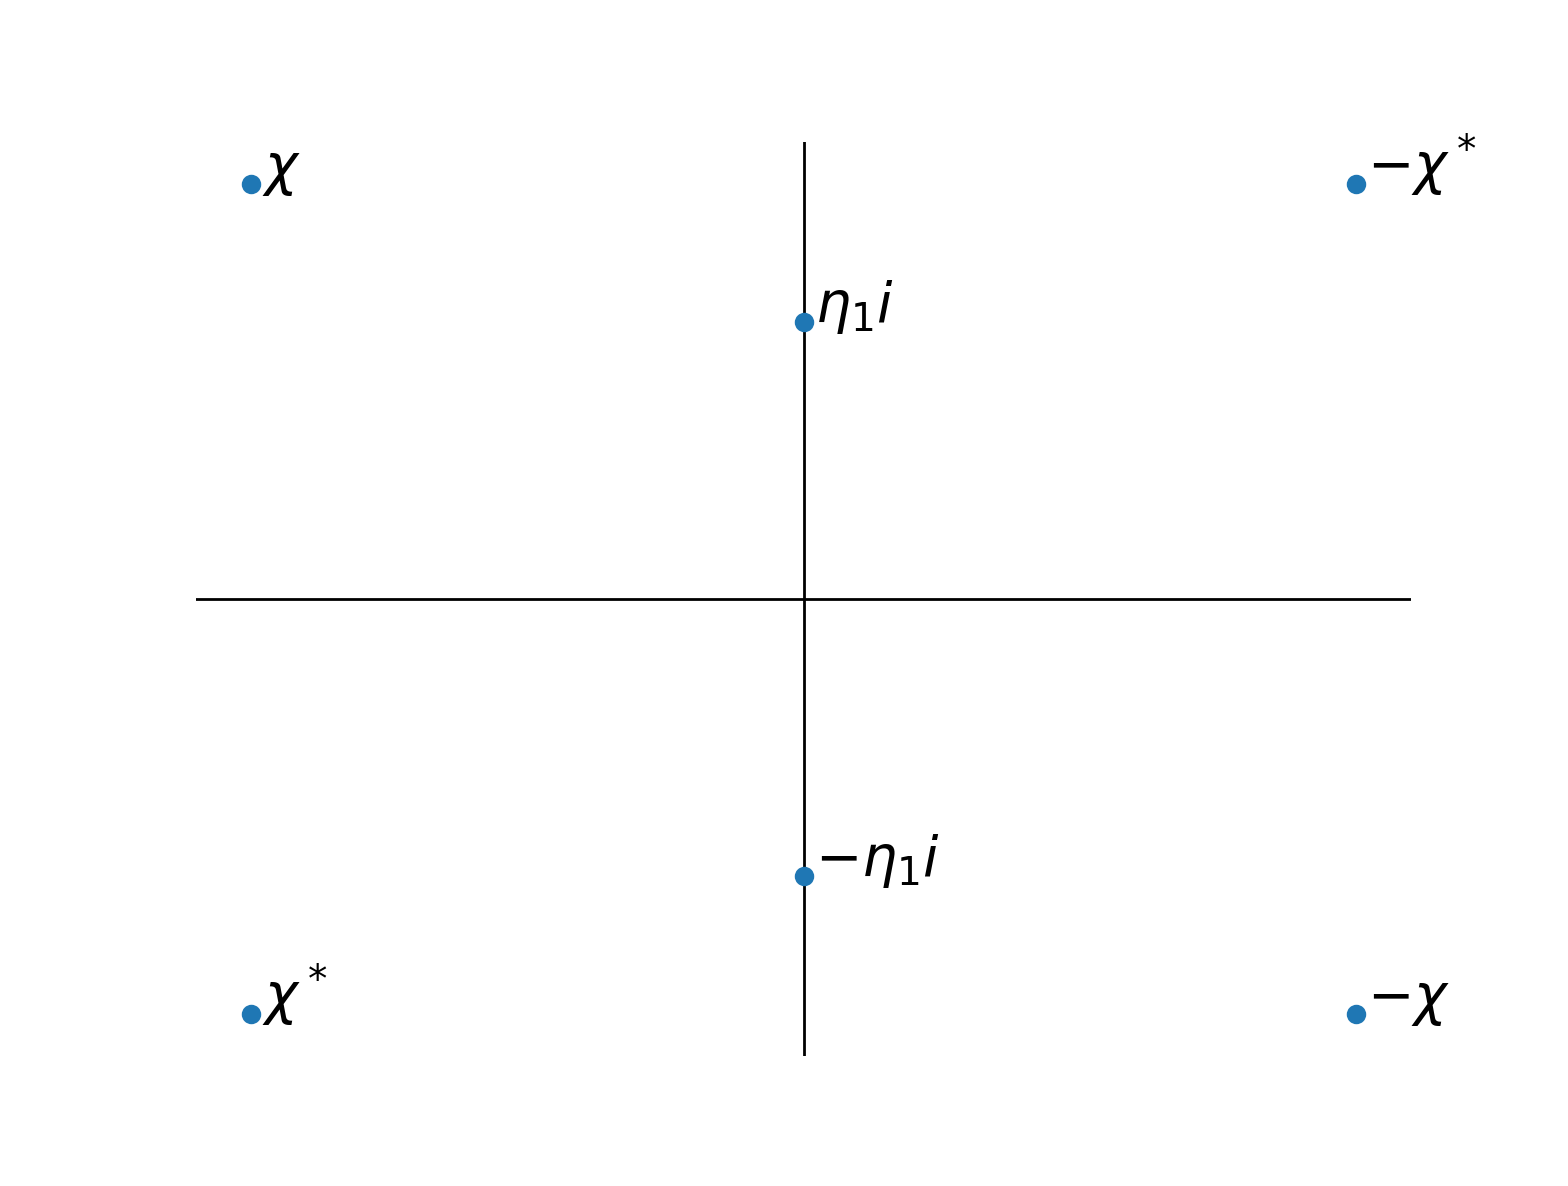
\includegraphics[width=0.5\textwidth]{pole_structure}
	\caption{\label{fig:pole_structure} The pole structure of the auto-correlation of the GLE Green's function $F(t)$ with an exponential memory kernel.}
\end{figure}

$\int\frac{dw}{2\pi} g\left(\omega\right) \left|\tilde{F}\left(\omega\right)\right|^2$ may now be evaluated using the residue theorem (closing the contour at $i\omega\rightarrow\infty$) provided that $g$ does not grow too fast as $\Im(\omega)\rightarrow\infty$. Assuming $g(\omega)$ has no poles and that $g(-\omega^*)=g(\omega)^*$ (which is useful for the purposes of this report),
\begin{equation}
	\int\frac{dw}{2\pi} g\left(\omega\right) \left|\tilde{F}\left(\omega\right)\right|^2 =  -\frac{1}{2 \tau^{2}}\left(\frac{1}{2 \chi' \chi''} \operatorname{Re}\left(\frac{g(\chi)}{\chi\left(\chi^{2}+\eta_{1}^{2}\right)}\right)+\frac{g(i\eta_{1})}{\left(|\chi|^{2}+n_{1}^{2}\right)^{2} \eta_{1}}\right) \label{eqn:integral_over_CF}
\end{equation}

\subsection{Evaluating the ISF and Energy Auto-correlation Function for an Exponential Memory Kernel}

Using equation \ref{eqn:integral_over_CF} the results derived in Section \ref{isf_gle_well} and \ref{kinetic_autocorrelation} can be evaluated for an exponential memory kernel $K(t)=\frac{1}{\tau}e^{-\frac{t}{\tau}}$. Substituting the expressions for the ISF and kinetic energy auto-correlation into equation \ref{eqn:integral_over_CF} and simplifying results in,
\begin{equation}
	ISF\left(\Delta \vec{K}, t\right) = ISF\left(\Delta \vec{K}, \infty\right) \exp\left(\frac{-\sigma^2\left|\Delta \vec{K}\right|^2}{2m^2\tau^2}\left(\frac{e^{-\chi''t}}{2\chi'\chi''}\operatorname{Re}\left(\frac{e^{i\chi't}}{\chi\left(\chi^2+\eta_1^2\right)}\right) + \frac{e^{-\eta_1t}}{\left(\left|\chi\right|^2+\eta_1^2\right)^2\eta_1}\right)\right) \label{isf_exp}
\end{equation}
\begin{equation}
	\left<E(0)E(t)\right>=\left<E(0)E(\infty)\right> + \frac{\sigma^4}{4\tau^4m^2}\left(\frac{e^{-\chi''t}}{2\chi'\chi''}\operatorname{Re}\left(\frac{\chi e^{i\chi't}}{\chi^2+\eta_1^2}\right) + \frac{\eta_1e^{-\eta_1 t}}{\left(\left|\chi\right|^2 + \eta_1^2\right)^2} \right)^2
\end{equation}
$$
\left<E(0)E(\infty)\right> = \frac{\sigma^4}{4\tau^4m^2}\left(\frac{1}{2\chi'\chi''}\operatorname{Re}\left(\frac{\chi}{\chi^2+\eta_1^2}\right) - \frac{\eta_1}{\left(\left|\chi\right|^2 + \eta_1^2\right)^2} \right)^2
$$

Where $\chi=:\chi'+\chi''i$.


\bibliographystyle{abbrv}
\bibliography{bibliography}

\end{document}
